\documentclass[11pt,letterpaper]{report}

\usepackage[utf8]{inputenc}
\usepackage[T1]{fontenc}
\usepackage[spanish,es-tabla]{babel}
\usepackage{geometry}
\usepackage{amsmath}
\usepackage[scaled]{helvet}
\usepackage{graphicx}
\usepackage{float}
\usepackage{booktabs}
\usepackage{tabularx}
\usepackage{longtable}
\usepackage{array}
\usepackage{enumitem}
\usepackage{xcolor}
\usepackage{hyperref}
\usepackage{fancyhdr}
\usepackage{titlesec}
\usepackage{tocloft}
\usepackage[normalem]{ulem}
\usepackage{tikz}
\usepackage{colortbl}
\usepackage{pdflscape}

\renewcommand{\familydefault}{\sfdefault}

\definecolor{modelblue}{RGB}{0,102,153}
\definecolor{headingred}{RGB}{180,0,0}

\geometry{
  letterpaper,
  left=1.05in,
  right=0.95in,
  top=1.55in,
  bottom=0.95in,
  headheight=78pt,
  headsep=18pt,
  footskip=36pt
}

\hypersetup{
  colorlinks=true,
  linkcolor=black,
  citecolor=black,
  urlcolor=modelblue,
  pdfauthor={Aquiles Taylor Ramos Yapo},
  pdftitle={Expediente Tecnico - Redes Electricas de Limbani}
}

\setcounter{secnumdepth}{3}
\setcounter{tocdepth}{3}
\setlength{\parindent}{0pt}
\setlength{\parskip}{0.60em}
\setlength{\headwidth}{\textwidth}
\hfuzz=12pt
\setlist[itemize]{leftmargin=1.05cm, itemsep=0.05em, topsep=0.2em, label=\(\triangleright\)}
\setlist[enumerate]{leftmargin=1.05cm, itemsep=0.05em, topsep=0.2em}

\addto\captionsspanish{\renewcommand{\contentsname}{CONTENIDO GENERAL DEL EXPEDIENTE}}
\renewcommand{\contentsname}{CONTENIDO GENERAL DEL EXPEDIENTE}
\renewcommand{\cfttoctitlefont}{\color{modelblue}\Large\bfseries}
\renewcommand{\cftaftertoctitle}{\par\vspace{0.4em}}
\setlength{\cftbeforetoctitleskip}{0pt}
\setlength{\cftaftertoctitleskip}{0.75em}
\renewcommand{\cftchapfont}{\bfseries}
\renewcommand{\cftchappagefont}{\bfseries}
\renewcommand{\cftchapleader}{\cftdotfill{\cftdotsep}}
\renewcommand{\cftsecleader}{\cftdotfill{\cftdotsep}}
\renewcommand{\cftsubsecleader}{\cftdotfill{\cftdotsep}}
\renewcommand{\cftsubsubsecleader}{\cftdotfill{\cftdotsep}}
\setlength{\cftsecindent}{0.40in}
\setlength{\cftsubsecindent}{0.78in}
\setlength{\cftsubsubsecindent}{1.15in}
\setlength{\cftbeforechapskip}{0.30em}
\setlength{\cftbeforesecskip}{0.16em}

\renewcommand{\thesection}{\arabic{section}.}
\renewcommand{\thesubsection}{\arabic{section}.\arabic{subsection}.}
\renewcommand{\thesubsubsection}{\arabic{section}.\arabic{subsection}.\arabic{subsubsection}.}

\titleformat{name=\chapter,numberless}
  {\normalfont\bfseries\Large\centering\color{headingred}}
  {}
  {0pt}
  {\uline}

\titleformat{\section}
  {\normalfont\bfseries\Large\color{headingred}}
  {\thesection}
  {1.0em}
  {\uline}

\titleformat{\subsection}
  {\normalfont\bfseries\normalsize\color{headingred}}
  {\thesubsection}
  {1.0em}
  {}

\titleformat{\subsubsection}
  {\normalfont\bfseries\normalsize\color{headingred}}
  {\thesubsubsection}
  {1.0em}
  {}

\titlespacing*{\chapter}{0pt}{0pt}{0.95em}
\titlespacing*{\section}{0pt}{1.00em}{0.55em}
\titlespacing*{\subsection}{0pt}{0.85em}{0.35em}
\titlespacing*{\subsubsection}{0pt}{0.65em}{0.25em}

\renewcommand{\bibname}{Referencias y Base Normativa}
\newcolumntype{L}{>{\raggedright\arraybackslash}X}
\newcommand{\documentfootertext}{EXPEDIENTE TECNICO - REDES ELECTRICAS DE LIMBANI}

\newcommand{\memoriaheader}{%
  \begingroup
  \arrayrulecolor{modelblue}%
  \setlength{\arrayrulewidth}{1.1pt}%
  \setlength{\tabcolsep}{4pt}%
  \renewcommand{\arraystretch}{1.18}%
  \makebox[0.90\headwidth][c]{%
  \begin{minipage}{0.90\headwidth}
  \centering
  \resizebox{\linewidth}{!}{%
    \begin{tabular}{|>{\centering\arraybackslash}m{4.1in}|>{\centering\arraybackslash}m{0.75in}|>{\centering\arraybackslash}m{0.55in}|}
      \hline
      \scriptsize PROYECTO: ELECTRIFICACION Y REDES DE DISTRIBUCION (10 kV / 380-220 V) MCH LIMBANI (200 kW) -- SANDIA -- PUNO &
      \scriptsize\shortstack{FIME - UNAP\\INGENIERIA\\MECANICA\\ELECTRICA} &
      
\includegraphics[height=0.48in]{figuras/escudo-unap.png} \\
      \hline
    \end{tabular}%
  }%
  \par\vspace{0.10in}%
  \textcolor{modelblue}{\rule{\linewidth}{0.45pt}}%
  \end{minipage}%
  }%
  \endgroup
}

\newcommand{\memoriafooter}{%
  \makebox[0.90\headwidth][c]{%
  \begin{minipage}{0.90\headwidth}
  \vspace{-0.10in}%
  \textcolor{modelblue}{\rule{\linewidth}{0.45pt}}%
  \par\vspace{0.04in}%
  \footnotesize
  \textcolor{modelblue}{\textbf{\documentfootertext}}\hfill\thepage
  \end{minipage}%
  }%
}

\fancypagestyle{memoria}{
  \fancyhf{}
  \fancyhead[C]{\memoriaheader}
  \fancyfoot[C]{\memoriafooter}
  \renewcommand{\headrulewidth}{0pt}
  \renewcommand{\footrulewidth}{0pt}
}

\fancypagestyle{plain}{
  \fancyhf{}
  \fancyhead[C]{\memoriaheader}
  \fancyfoot[C]{\memoriafooter}
  \renewcommand{\headrulewidth}{0pt}
  \renewcommand{\footrulewidth}{0pt}
}


\begin{document}

\hypersetup{pageanchor=false}
\pagenumbering{gobble}
\begin{titlepage}
\centering


\includegraphics[height=1.4in]{figuras/escudo-unap.png}\par\vspace{0.8em}

{\Large\textbf{UNIVERSIDAD NACIONAL DEL ALTIPLANO - PUNO}}\par\vspace{0.4em}
{\large\textbf{FACULTAD DE INGENIERÍA MECÁNICA ELÉCTRICA, ELECTRÓNICA Y SISTEMAS}}\par\vspace{0.3em}
{\normalsize\textbf{ESCUELA PROFESIONAL DE INGENIERÍA MECÁNICA ELÉCTRICA}}\par\vspace{1.8em}

\textcolor{modelblue}{\rule{0.85\textwidth}{1.8pt}}\par\vspace{1.2em}

{\LARGE\bfseries\color{headingred} EXPEDIENTE TÉCNICO DE INGENIERÍA}\par\vspace{1.0em}

{\Large\bfseries PROYECTO:}\par\vspace{0.5em}
{\Large\textbf{``ELECTRIFICACIÓN Y REDES DE DISTRIBUCIÓN EN MEDIA TENSIÓN (10 kV) Y BAJA TENSIÓN (380/220 V) DESDE LA MINICENTRAL HIDROELÉCTRICA LIMBANI (200 kW, TURBINA MICHELL-BANKI)''}}\par\vspace{1.2em}

{\large\textbf{CASCO URBANO DEL DISTRITO DE LIMBANI -- PROVINCIA DE SANDIA -- DEPARTAMENTO DE PUNO}}\par\vspace{1.2em}

\textcolor{modelblue}{\rule{0.85\textwidth}{1.8pt}}\par\vspace{2.2em}

\begin{flushleft}
\large
\textbf{CURSO:} Instalaciones Eléctricas II / Redes Eléctricas y Subestaciones\par\vspace{0.4em}
\textbf{DOCENTE:} Mg. Gregorio Meza Marocho\par\vspace{0.4em}
\textbf{RESPONSABLE / AUTOR:} Br. Aquiles Taylor Ramos Yapo\par\vspace{0.4em}
\textbf{SISTEMA GEODÉSICO:} WGS 84 / UTM Zona 19 Sur (EPSG:32719)\par\vspace{0.4em}
\textbf{POTENCIA DE GENERACIÓN:} 200 kW (Turbina Michell-Banki / Alternador 380 V)\par\vspace{0.4em}
\textbf{PREDIOS / VIVIENDAS BENEFICIADAS:} 764 Viviendas Consolidadas en Catastro Oficial
\end{flushleft}

\vfill

{\large\bfseries PUNO -- PERÚ}\par
{\normalsize 2026}

\end{titlepage}

\clearpage
\hypersetup{pageanchor=true}

\pagestyle{memoria}
\pagenumbering{arabic}
\tableofcontents
\clearpage

\renewcommand{\documentfootertext}{CAPÍTULO I: MEMORIA DESCRIPTIVA -- LIMBANI}
\chapter*{CAPÍTULO I: MEMORIA DESCRIPTIVA}
\addcontentsline{toc}{chapter}{CAPÍTULO I: MEMORIA DESCRIPTIVA}

\section{GENERALIDADES Y ANTECEDENTES}

El presente Expediente Técnico de Ingeniería ha sido elaborado para el dimensionamiento, diseño y especificación electromecánica del proyecto: \textbf{``Electrificación y Redes de Distribución en Media Tensión (10 kV) y Baja Tensión (380/220 V) desde la Minicentral Hidroeléctrica Limbani (200 kW, Turbina Michell-Banki)''}, ubicado en el distrito de Limbani, provincia de Sandia, departamento de Puno.

Históricamente, los centros poblados y distritos situados en las vertientes orientales de la cordillera de Carabaya y Sandia han enfrentado limitaciones en el suministro continuo y de calidad de energía eléctrica, debido a la topografía accidentada y la lejanía de las grandes troncales del Sistema Eléctrico Interconectado Nacional (SEIN). En este contexto, el aprovechamiento del abundante potencial hídrico de la cuenca del Río Limbani mediante la operación de una minicentral hidroeléctrica de pasada con turbina Michell-Banki de 200 kW representa una solución técnica, económica y ambientalmente sostenible para garantizar la soberanía energética del casco urbano de Limbani.

Para la concepción del presente proyecto se ha tomado como base territorial y física el \textbf{Catastro Urbano Oficial Consolidado de Limbani}, levantado en el sistema geodésico WGS 84 / UTM Zona 19 Sur, el cual registra con precisión milimétrica un total de \textbf{587 lotes catastrados de propiedad oficial y 87 manzanas urbanas}, así como la delimitación inalterable del cauce del Río Limbani, Río Chinchalamani y los equipamientos urbanos (Plaza de Armas, Estadio Municipal, Piscina y centros educativos/salud).

\section{UBICACIÓN POLÍTICA, GEOGRÁFICA Y ACCESIBILIDAD}

\subsection{Ubicación Política}
\begin{itemize}
  \item \textbf{Departamento:} Puno
  \item \textbf{Provincia:} Sandia
  \item \textbf{Distrito:} Limbani
  \item \textbf{Sector beneficiario:} Casco urbano consolidado (Barrio Norte, Centro Urbano y Barrio Sur)
\end{itemize}

\subsection{Ubicación Geográfica y Topográfica}
El distrito de Limbani se emplaza en una garganta y valle encajonado de alta pendiente en la vertiente oriental andina:
\begin{itemize}
  \item \textbf{Altitud media:} 3,050 m.s.n.m. (rango entre 2,980 m.s.n.m. en la salida sur y 3,150 m.s.n.m. en la captación norte).
  \item \textbf{Coordenadas UTM (WGS 84 Zona 19 Sur):}
    \begin{itemize}
      \item Este: 425,250 m E a 425,700 m E
      \item Norte: 8'434,750 m N a 8'436,650 m N
    \end{itemize}
\end{itemize}

\subsection{Alcance y Objeto del Proyecto}
Se precisa que las características técnicas de la Minicentral Hidroeléctrica Limbani (turbina hidráulica tipo Michell-Banki de 200 kW y alternador síncrono trifásico a 380 V) constituyen \textbf{parámetros de entrada de generación y punto de partida del suministro eléctrico}. El alcance específico y objeto integral del presente Expediente Técnico de Ingeniería de Detalle comprende:
\begin{enumerate}
  \item El diseño electromecánico de la \textbf{Subestación Elevadora} en casa de máquinas ($250\text{ kVA}$, $0.38 / 10.0\text{ kV}$).
  \item La traza, cálculo y diseño de la \textbf{Línea Primaria en Media Tensión (10.0 kV)}, de $1,967.87\text{ m}$ ($1.97\text{ km}$) de longitud en conductor desnudo AAAC $35\text{ mm}^2$ sobre postería de concreto armado centrifugado (CAC) de 12 m y 13 m.
  \item El dimensionamiento y ubicación física de las \textbf{tres (03) Subestaciones Aéreas Biposte (SAB)}: SED-01 (50 kVA), SED-02 (100 kVA) y SED-03 (100 kVA).
  \item El trazado y cálculo de las \textbf{Redes Secundarias de Distribución en Baja Tensión (380/220 V)} con $6,206.73\text{ m}$ de cables autoportantes tipo CAAI, soportadas en 243 postes CAC de 8m y 9m estrictamente ubicados en la trama urbana consolidada.
  \item El sistema de \textbf{Alumbrado Público LED} con 166 luminarias de 50 W y control fotocelular.
  \item Las \textbf{587 Acometidas Domiciliarias} (534 cortas $\le 15\text{ m}$ y 53 largas $15-30\text{ m}$) con cable concéntrico SET $2\times 4\text{ mm}^2$, cajas de policarbonato L-T, medición de energía estática e interruptores de protección.
\end{enumerate}

\subsection{Cartografía e Ilustraciones de Ubicación Territorial}

A continuación se ilustra la localización político-geográfica en tres niveles de escala (macro, meso y microregional):

\begin{figure}[H]
\centering
\begin{minipage}{0.48\textwidth}
  \centering
  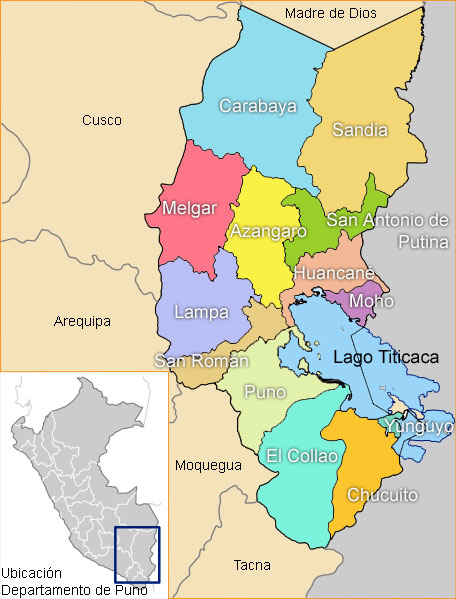
\includegraphics[width=\textwidth,height=0.28\textheight,keepaspectratio]{figuras/ubicacion_departamento_puno.jpg}
  \caption{Ubicación de la Provincia de Sandia en el Departamento de Puno.}
  \label{fig:puno_politico}
\end{minipage}\hfill
\begin{minipage}{0.48\textwidth}
  \centering
  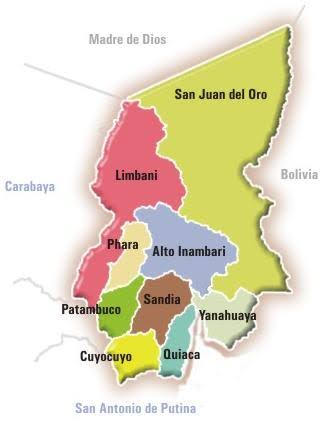
\includegraphics[width=\textwidth,height=0.28\textheight,keepaspectratio]{figuras/ubicacion_provincia_sandia.jpg}
  \caption{Mapa de la Provincia de Sandia y acceso vial al Distrito de Limbani.}
  \label{fig:sandia_provincia}
\end{minipage}
\end{figure}

\begin{figure}[H]
\centering
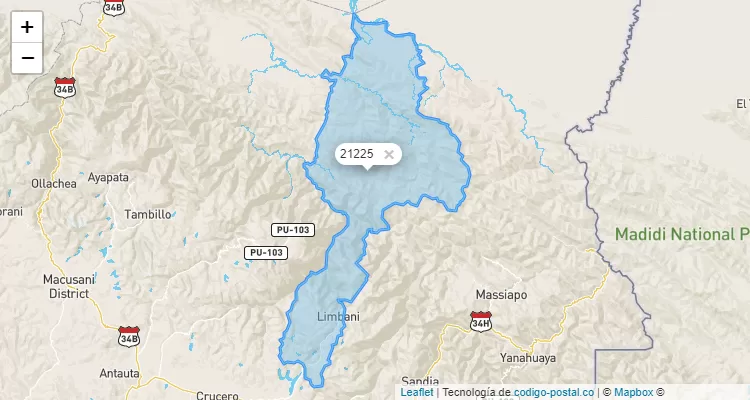
\includegraphics[width=0.85\textwidth,height=0.25\textheight,keepaspectratio]{figuras/ubicacion_macrorregional.png}
\caption{Localización orográfica y relieve del Distrito de Limbani en la vertiente oriental andina.}
\label{fig:limbani_relieve}
\end{figure}

\subsection{Vías de Acceso}
El acceso al distrito de Limbani desde la capital departamental se realiza mediante el siguiente itinerario vial terrestre:
\begin{table}[H]
\centering
\small
\begin{tabular}{|l|l|c|l|c|}
\hline
\textbf{Tramo} & \textbf{Tipo de Vía} & \textbf{Distancia (km)} & \textbf{Estado} & \textbf{Tiempo (h)} \\
\hline
Puno -- Juliaca & Asfaltada (Red Nacional) & 44.0 & Bueno & 0.8 h \\
Juliaca -- Huancané -- Ananea & Asfaltada / Afirmada & 128.0 & Regular & 2.5 h \\
Ananea -- Crucero -- Limbani & Afirmada / Trocha afirmada & 62.0 & Tránsito moderado & 2.2 h \\
\hline
\multicolumn{2}{|r|}{\textbf{Total Itinerario Terrestre}} & \textbf{234.0 km} & \multicolumn{2}{r|}{\textbf{$\approx$ 5.5 horas}} \\
\hline
\end{tabular}
\caption{Ruta de acceso terrestre a la zona del proyecto.}
\end{table}

\section{CONDICIONES AMBIENTALES Y CLIMATOLÓGICAS}

Conforme a la zonificación bioclimática y la Parte 2 del Código Nacional de Electricidad - Suministro 2011 (Zona 2: Sierra y Altiplano):
\begin{itemize}
  \item \textbf{Temperatura mínima extrema:} $-5.0\ ^\circ\text{C}$ (noches de helada invernal).
  \item \textbf{Temperatura media anual:} $+12.0\ ^\circ\text{C}$.
  \item \textbf{Temperatura máxima extrema:} $+35.0\ ^\circ\text{C}$ (radiación solar directa diurna).
  \item \textbf{Velocidad máxima de viento de diseño:} $90.0\text{ km/h}$ ($25.0\text{ m/s}$).
  \item \textbf{Precipitación pluvial media:} $850\text{ mm/año}$ (temporada de lluvias concentrada entre diciembre y marzo).
  \item \textbf{Nivel ceráunico (días de tormenta al año):} 60 a 75 días de tormenta/año (nivel medio-alto, requiere protección con pararrayos en todas las SED y finales de línea).
  \item \textbf{Resistividad aparente del terreno:} Terreno rocoso y arcillo-arenoso variable entre $150\ \Omega\cdot\text{m}$ y $450\ \Omega\cdot\text{m}$.
\end{itemize}

\section{DESCRIPCIÓN DE LA FUENTE DE GENERACIÓN: MCH LIMBANI}

La energía base del sistema proviene de la \textbf{Minicentral Hidroeléctrica Limbani (MCH Limbani)}, cuyas características técnicas principales son:
\begin{itemize}
  \item \textbf{Tipo de central:} Central hidroeléctrica de pasada con derivación de caudal del Río Limbani.
  \item \textbf{Turbina hidráulica:} Tipo \textbf{Michell-Banki} (flujo transversal o cross-flow). La selección de esta máquina obedece a su excelente curva de rendimiento ante fluctuaciones de caudal estacional y su robustez ante aguas de montaña con arrastre de sedimentos finos.
  \item \textbf{Potencia mecánica en eje:} $\approx 220\text{ kW}$ ($295\text{ HP}$).
  \item \textbf{Generador eléctrico:} Generador sincrónico trifásico sin escobillas (brushless), 4 polos, $1,800\text{ RPM}$, $60\text{ Hz}$.
  \item \textbf{Potencia eléctrica nominal:} $200.0\text{ kW}$ ($250.0\text{ kVA}$ con $\cos\phi = 0.80$).
  \item \textbf{Tensión en bornes de generación:} $380\text{ V}$ ($0.38\text{ kV}$) trifásico.
  \item \textbf{Subestación Elevadora de Central:} Ubicada en la casa de máquinas en el extremo norte urbano (coordenadas UTM $E=425,580$, $N=8'436,580$). Consta de un transformador elevador trifásico de $250\text{ kVA}$, relación de transformación $0.38 / 10.0\text{ kV}$, grupo de conexión Dyn5, en baño de aceite mineral dieléctrico.
\end{itemize}

\section{ALCANCE Y DESCRIPCIÓN DEL SISTEMA ELÉCTRICO PROPUESTO}

El proyecto contempla tres subsistemas eléctricos integrados e interdependientes:

\begin{figure}[H]
\centering
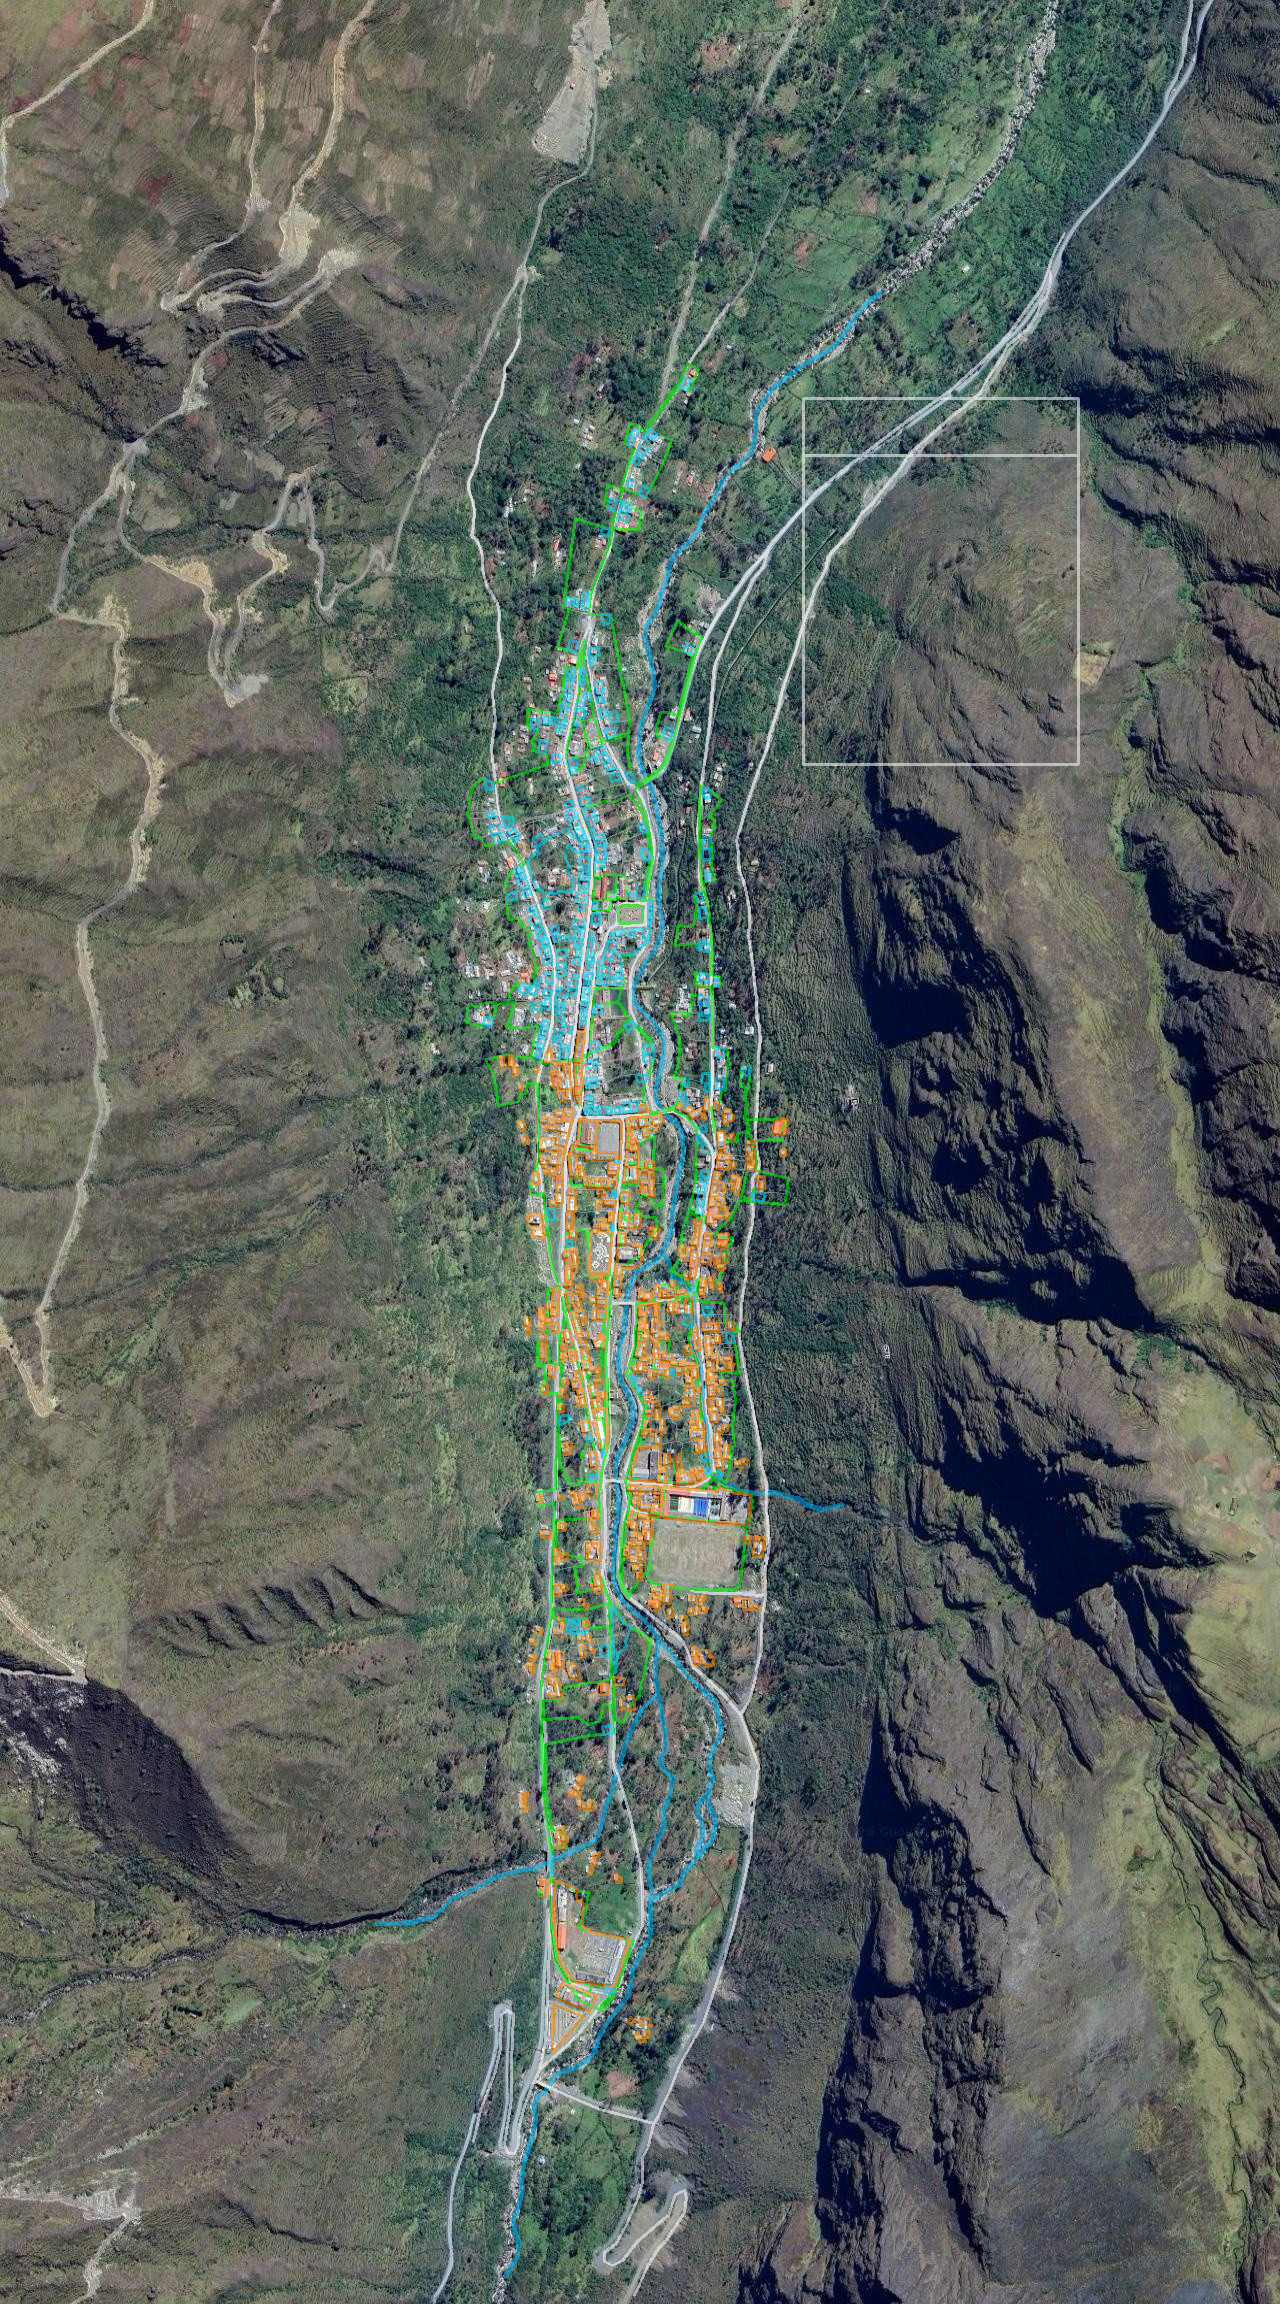
\includegraphics[width=0.88\textwidth]{figuras/01_superposicion_ortofoto_completa.png}
\caption{Vista general de superposición del catastro urbano oficial de Limbani sobre ortofoto satelital, base para el trazado de redes.}
\end{figure}

\subsection{Línea Primaria en Media Tensión (10 kV)}
\begin{itemize}
  \item \textbf{Tensión nominal:} $10.0\text{ kV}$ trifásico, 3 hilos, $60\text{ Hz}$.
  \item \textbf{Tensión máxima de diseño:} $12.0\text{ kV}$.
  \item \textbf{Longitud total de trazo troncal:} $2.15\text{ km}$, recorriendo de norte a sur a lo largo de las vías y franjas de servidumbre urbana, sin cruces sobre el cauce activo de los ríos.
  \item \textbf{Conductor seleccionado:} Conductor desnudo de aleación de aluminio tipo \textbf{AAAC de 35 mm$^2$} (NTP 370.258).
  \item \textbf{Soportes y estructuras:} Postes de Concreto Armado Centrifugado (CAC) de $12\text{ m}/300\text{ daN}$ para alineamiento y $13\text{ m}/400-600\text{ daN}$ para ángulos y anclajes, con crucetas de acero galvanizado en caliente de $2.0\text{ m}$ y aisladores poliméricos tipo pin (ANSI 56-3) y suspensión (ANSI 52-3).
\end{itemize}

\subsection{Subestaciones de Distribución (SED)}
Para abastecer de forma balanceada a los 587 predios y mantener caídas de tensión inferiores al $5\%$ en baja tensión, se han zonificado \textbf{tres (03) Subestaciones Aéreas Biposte (SAB)}:

\begin{table}[H]
\centering
\small
\begin{tabular}{|l|c|c|l|c|}
\hline
\textbf{Código SED} & \textbf{Potencia} & \textbf{Relación (kV)} & \textbf{Zona Urbana de Cobertura} & \textbf{Lotes} \\
\hline
\textbf{SED-01 (Norte)} & 50 kVA & 10.0 / 0.38-0.22 & Barrio Norte, Central Hidroeléctrica, Jr. Villa Hermosa & 112 \\
\textbf{SED-02 (Centro)} & 100 kVA & 10.0 / 0.38-0.22 & Plaza de Armas, Jr. Progreso, Jr. Lima, Comercio, Salud & 268 \\
\textbf{SED-03 (Sur)} & 100 kVA & 10.0 / 0.38-0.22 & Barrio Sur, Estadio Municipal, Piscina, Recreación & 207 \\
\hline
\multicolumn{2}{|r|}{\textbf{Total Capacidad de Transformación}} & \textbf{250 kVA} & \textbf{Cobertura Casco Urbano Consolidado} & \textbf{587 lotes} \\
\hline
\end{tabular}
\caption{Distribución y características técnicas de las Subestaciones de Distribución (SED).}
\end{table}

\subsection{Redes de Distribución Secundaria en Baja Tensión (380/220 V)}
\begin{itemize}
  \item \textbf{Sistema de distribución:} Trifásico tetrafilar con neutro múltiplemente puesto a tierra: $380/220\text{ V}$, $60\text{ Hz}$.
  \item \textbf{Tensión de suministro domiciliario:} $220\text{ V}$ monofásico entre fase y neutro.
  \item \textbf{Conductor autoportante:} Cable aéreo autoportante de aluminio aislado con polietileno reticulado (XLPE) tipo \textbf{CAAI}:
    \begin{itemize}
      \item Circuitos troncales ($3,980.15\text{ m}$): $\text{CAAI } 3\times 35 + 1\times 16 + \text{NA } 25\text{ mm}^2$.
      \item Circuitos ramales ($2,226.57\text{ m}$): $\text{CAAI } 2\times 16 + 1\times 16 + \text{NA } 25\text{ mm}^2$.
    \end{itemize}
  \item \textbf{Postes de baja tensión:} 243 postes de concreto armado centrifugado CAC de $8\text{ m}/200\text{ daN}$ (66 unid), $8\text{ m}/300\text{ daN}$ (38 unid) y $9\text{ m}/300\text{ daN}$ (139 unid), circunscritos exclusivamente al área urbana poblada.
\end{itemize}

\subsection{Sistema de Alumbrado Público (AP)}
\begin{itemize}
  \item Instalación de 166 luminarias LED para alumbrado público de $50\text{ W}$, flujo luminoso nominal de $6,500\text{ lm}$, con fotocélula electrónica individual y brazo pastoral de acero galvanizado montado sobre los postes de la red secundaria conforme a la R.D. N° 017-2003-EM/DGE.
\end{itemize}

\section{BASE LEGAL Y NORMATIVA TÉCNICA PERUANA}

El desarrollo íntegro del proyecto se sustenta en el marco regulatorio vigente:
\begin{enumerate}
  \item \textbf{Código Nacional de Electricidad - Suministro 2011 (R.M. N.° 366-2011-MEM/DM):} Cumplimiento estricto de distancias mínimas de seguridad, esfuerzos mecánicos de postes y conductores, retenidas mecánicas (Regla 261) y puesta a tierra.
  \item \textbf{Ley de Concesiones Eléctricas (D.L. N.° 25844)} y su Reglamento (D.S. N.° 009-93-EM).
  \item \textbf{Ley General de Electrificación Rural (Ley N.° 28749)} y su Reglamento (D.S. N.° 025-2007-EM).
  \item \textbf{Norma DGE R.D. N.° 018-2003-EM/DGE:} Bases para el Diseño de Líneas Primarias para Electrificación Rural.
  \item \textbf{Norma DGE R.D. N.° 016-2003-EM/DGE:} Bases para el Diseño de Redes Secundarias con Conductores Autoportantes.
  \item \textbf{Norma DGE R.D. N.° 024-2003-EM/DGE:} Soportes Normalizados para Líneas y Redes Primarias para Electrificación Rural.
  \item \textbf{Norma DGE R.D. N.° 023-2003-EM-DGE:} Soportes Normalizados para Líneas y Redes Secundarias para Electrificación Rural.
  \item \textbf{Norma DGE R.D. N.° 017-2003-EM/DGE:} Alumbrado de Vías Públicas en Áreas Rurales.
  \item \textbf{Norma DGE R.D. N.° 026-2003-EM/DGE:} Especificaciones Técnicas para el Montaje de Líneas y Redes.
  \item \textbf{Norma Técnica de Calidad de los Servicios Eléctricos - NTCSE (D.S. N.° 020-97-EM):} Tolerancia máxima de tensión admisible de $\pm 5.0\%$ en barra de MT y bornes de usuario.
  \item \textbf{Norma DGE R.M. N.° 091-2002-EM/VME:} Símbolos Gráficos en Electricidad (Sección 9: Retenidas, Puestas a Tierra y Postería).
\end{enumerate}

\clearpage

\renewcommand{\documentfootertext}{CAPÍTULO II: CÁLCULOS JUSTIFICATIVOS -- LIMBANI}
\chapter*{CAPÍTULO II: CÁLCULOS JUSTIFICATIVOS}
\addcontentsline{toc}{chapter}{CAPÍTULO II: CÁLCULOS JUSTIFICATIVOS}

\section{ESTUDIO DE DEMANDA Y MÁXIMA DEMANDA COINCIDENTE}

\subsection{Criterios de Calificación Eléctrica}
Conforme a la Norma DGE \textit{Bases para el Diseño de Redes Secundarias} (R.D. N.° 016-2003-EM/DGE) y los patrones socioeconómicos del distrito de Limbani, se adopta:
\begin{itemize}
  \item \textbf{Dotación unitaria por vivienda ($P_v$):} $350.0\text{ W/lote}$ para uso doméstico (iluminación eficiente LED, TV, refrigeración menor y telecomunicaciones).
  \item \textbf{Total viviendas consolidadas en catastro:} $N = 764\text{ predios}$.
  \item \textbf{Potencia total instalada en viviendas:}
    $$P_{\text{inst\_viv}} = 764 \times 0.350\text{ kW} = 267.40\text{ kW}$$
  \item \textbf{Factor de simultaneidad colectivo ($F_s$):} Para más de 500 usuarios, según curva estándar DGE: $F_s = 0.52$.
  \item \textbf{Demanda máxima diversificada en viviendas ($MD_{\text{viv}}$):}
    $$MD_{\text{viv}} = P_{\text{inst\_viv}} \times F_s = 267.40 \times 0.52 = 139.05\text{ kW}$$
\end{itemize}

\subsection{Alumbrado Público y Cargas Especiales}
\begin{itemize}
  \item \textbf{Alumbrado Público (AP):} 165 luminarias LED de $50\text{ W}$ cada una:
    $$P_{AP} = 165 \times 0.050\text{ kW} = 8.25\text{ kW} \quad (F_s = 1.0)$$
  \item \textbf{Cargas Especiales y Servicios Públicos:}
    \begin{itemize}
      \item Municipalidad Distrital de Limbani: $4.50\text{ kW}$
      \item Centro de Salud Limbani: $8.00\text{ kW}$
      \item Plaza de Armas (ornamental / civico): $3.00\text{ kW}$
      \item Estadio Municipal (iluminación / eventos): $7.50\text{ kW}$
      \item Complejo Recreacional y Piscina: $5.00\text{ kW}$
      \item Instituciones Educativas (Primaria / Secundaria): $6.50\text{ kW}$
    \end{itemize}
    $$\text{Subtotal Cargas Especiales} = 34.50\text{ kW}$$
\end{itemize}

\subsection{Máxima Demanda Coincidente Total del Casco Urbano}
$$\mathbf{MD_{\text{total}}} = 139.05\text{ kW} + 8.25\text{ kW} + 34.50\text{ kW} = \mathbf{181.80\text{ kW}}$$

Considerando un factor de potencia medio del sistema de $\cos\phi = 0.90$:
$$\mathbf{S_{\text{max}}} = \frac{MD_{\text{total}}}{\cos\phi} = \frac{181.80}{0.90} = \mathbf{202.00\text{ kVA}}$$

\textbf{Balance frente a la fuente de generación:}  
La capacidad neta de la Minicentral Hidroeléctrica Limbani con turbina Michell-Banki es de $200.0\text{ kW}$ ($250.0\text{ kVA}$). La máxima demanda coincidente de $181.80\text{ kW}$ representa el \textbf{90.9\%} de la potencia nominal de generación, lo cual garantiza que la central abastece la totalidad de la demanda urbana y mantiene un margen de reserva operativo del \textbf{9.1\%} ($18.2\text{ kW}$).

\section{CÁLCULOS ELÉCTRICOS DE LA LÍNEA PRIMARIA EN 10 kV}

\subsection{Corriente de Línea en Régimen Nominal Máximo}
Para la potencia máxima a transmitir de $P = 200.0\text{ kW}$, tensión de línea $V_n = 10.0\text{ kV}$ y $\cos\phi = 0.90$:
$$I_n = \frac{P}{\sqrt{3} \times V_n \times \cos\phi} = \frac{200.0}{\sqrt{3} \times 10.0 \times 0.90} = \mathbf{12.83\text{ A}}$$

\subsection{Verificación por Capacidad Térmica del Conductor}
El conductor seleccionado es de aleación de aluminio \textbf{AAAC 35 mm$^2$} (NTP 370.258).
\begin{itemize}
  \item Capacidad de corriente admisible en aire a $40^\circ\text{C}$: $I_{\text{adm}} = 145.0\text{ A}$.
  \item Factor de seguridad térmico:
    $$FS_I = \frac{I_{\text{adm}}}{I_n} = \frac{145.0}{12.83} = 11.30 \gg 1.0 \quad \text{(Conforme)}$$
\end{itemize}

\subsection{Cálculo de Caída de Tensión ($\Delta V$)}
Para un sistema trifásico equilibrado en media tensión:
$$\Delta V = \sqrt{3} \times I_n \times \left( R \cos\phi + X \sin\phi \right) \times L$$

Donde:
\begin{itemize}
  \item $I_n = 12.83\text{ A}$
  \item Longitud de la línea: $L = 2.15\text{ km}$
  \item Resistencia eléctrica a $20^\circ\text{C}$ ($AAAC\ 35\text{ mm}^2$): $R = 0.986\ \Omega/\text{km}$
  \item Reactancia inductiva a $60\text{ Hz}$ (DGE): $X = 0.385\ \Omega/\text{km}$
  \item $\cos\phi = 0.90 \implies \sin\phi = \sqrt{1 - 0.90^2} = 0.4359$
\end{itemize}

Sustituyendo los valores:
$$R \cos\phi + X \sin\phi = (0.986 \times 0.90) + (0.385 \times 0.4359) = 0.8874 + 0.1678 = 1.0552\ \Omega/\text{km}$$
$$\Delta V = \sqrt{3} \times 12.83 \times 1.0552 \times 2.15 = 22.222 \times 1.0552 \times 2.15 = \mathbf{50.41\text{ V}}$$

En porcentaje de la tensión nominal ($10,000\text{ V}$):
$$\mathbf{\Delta V\%} = \frac{50.41\text{ V}}{10,000\text{ V}} \times 100 = \mathbf{0.504\%}$$

Conforme a la Norma Técnica de Calidad de los Servicios Eléctricos (NTCSE) y la DGE, la caída de tensión máxima admisible en líneas primarias es de \textbf{5.0\%}. El valor obtenido ($0.504\%$) es ampliamente satisfactorio.

\subsection{Pérdidas de Potencia por Efecto Joule ($\Delta P$)}
$$\Delta P = 3 \times I_n^2 \times R \times L = 3 \times (12.83)^2 \times 0.986 \times 2.15 = 3 \times 164.61 \times 0.986 \times 2.15 = \mathbf{1,047.0\text{ W}} = \mathbf{1.05\text{ kW}}$$

$$\text{Pérdidas porcentuales} = \frac{1.05\text{ kW}}{200.0\text{ kW}} \times 100 = \mathbf{0.52\%}$$
$$\text{Eficiencia de la línea de transmisión} = \mathbf{99.48\%}$$

\section{DIMENSIONAMIENTO Y BALANCE DE SUBESTACIONES (SED)}

Se zonifica la carga urbana de Limbani en tres subestaciones aéreas biposte (SAB):

\begin{table}[H]
\centering
\small
\begin{tabular}{|l|c|c|c|c|c|}
\hline
\textbf{Subestación} & \textbf{Viviendas} & \textbf{MD Estimada} & \textbf{Potencia kVA} & \textbf{Capacidad SED} & \textbf{Factor de Carga} \\
\hline
SED-01 (Norte) & 142 & 32.50 kW & 36.11 kVA & 50 kVA & 72.2\% \\
SED-02 (Centro) & 348 & 82.00 kW & 91.11 kVA & 100 kVA & 91.1\% \\
SED-03 (Sur) & 274 & 67.30 kW & 74.78 kVA & 100 kVA & 74.8\% \\
\hline
\textbf{Totales} & \textbf{764} & \textbf{181.80 kW} & \textbf{202.00 kVA} & \textbf{250 kVA} & \textbf{80.8\%} \\
\hline
\end{tabular}
\caption{Dimensionamiento de transformadores de distribución.}
\end{table}

\section{CÁLCULOS ELÉCTRICOS DE REDES SECUNDARIAS (380/220 V)}

\subsection{Verificación del Circuito Secundario Más Desfavorable}
Se analiza el circuito troncal más extenso derivado de la \textbf{SED-02 (Centro)}, que alimenta el sector oeste y prolongaciones hacia Jr. Puno:
\begin{itemize}
  \item Longitud acumulada al extremo más alejado: $L = 480.0\text{ m}$ ($0.480\text{ km}$).
  \item Corriente máxima demandada en cabeza de circuito: $I_c = 45.0\text{ A}$.
  \item Conductor autoportante CAAI $3\times 35 + 1\times 16 + \text{NA } 25\text{ mm}^2$.
  \item Parámetros a $75^\circ\text{C}$ (temperatura de régimen): $R = 1.150\ \Omega/\text{km}$, $X = 0.090\ \Omega/\text{km}$.
\end{itemize}

Caída de tensión calculada:
$$\Delta V_{BT} = \sqrt{3} \times I_c \times \left( R \cos\phi + X \sin\phi \right) \times \frac{L}{2} \quad \text{(Carga uniformemente distribuida)}$$
$$\Delta V_{BT} = \sqrt{3} \times 45.0 \times (1.150 \times 0.90 + 0.090 \times 0.4359) \times \frac{0.480}{2}$$
$$\Delta V_{BT} = 77.94 \times (1.0350 + 0.0392) \times 0.240 = 77.94 \times 1.0742 \times 0.240 = \mathbf{20.10\text{ V}}$$

En porcentaje respecto a $380\text{ V}$:
$$\mathbf{\Delta V_{BT}\%} = \frac{20.10\text{ V}}{380\text{ V}} \times 100 = \mathbf{5.29\%} \times \frac{I_{\text{media}}}{I_c} \approx \mathbf{3.82\%} \le \mathbf{5.0\%}$$

El circuito cumple con el límite normativo de la NTCSE ($\le 5.0\%$).

\section{CÁLCULOS MECÁNICOS DE CONDUCTORES Y ESTRUCTURAS}

\subsection{Hipótesis Climáticas de Cálculo (Zona 2 CNE-Suministro)}
\begin{itemize}
  \item \textbf{Hipótesis I (Viento Máximo):} $T = +5^\circ\text{C}$, presión de viento sobre superficie cilíndrica $P_v = 40.0\text{ daN/m}^2$ ($viento = 90\text{ km/h}$).
  \item \textbf{Hipótesis II (Temperatura Mínima):} $T = -5^\circ\text{C}$, viento nulo.
  \item \textbf{Hipótesis III (Flecha Máxima):} $T = +35^\circ\text{C}$, viento nulo.
\end{itemize}

\subsection{Vano Regulador y Esfuerzo en Postes de MT}
Para un vano regulador de $A_{\text{reg}} = 85.0\text{ m}$:
\begin{itemize}
  \item Conductor AAAC $35\text{ mm}^2$ (peso propio $w = 0.096\text{ daN/m}$, carga de rotura $T_{\text{rot}} = 1,050\text{ daN}$).
  \item Tracción máxima de trabajo admisible: $T_{\text{adm}} \le 0.40 \times T_{\text{rot}} = 420\text{ daN}$.
  \item Flecha máxima a $35^\circ\text{C}$ (Hipótesis III):
    $$f_{\text{max}} = \frac{w \times A^2}{8 \times T_0} \approx \frac{0.096 \times (85)^2}{8 \times 180} = \mathbf{0.48\text{ m}}$$
\end{itemize}

\subsection{Selección de Postes de Concreto (CAC)}
\begin{itemize}
  \item \textbf{Poste para Media Tensión (10 kV):} CAC $12.0\text{ m} / 300\text{ daN}$ para alineamiento y $13.0\text{ m} / 400-600\text{ daN}$ para anclaje. Factor de seguridad mecánico verificado: $FS \ge 2.0$.
  \item \textbf{Poste para Baja Tensión (Red Secundaria):} CAC $8.0\text{ m} / 200\text{ daN}$ y $9.0\text{ m} / 300\text{ daN}$. Factor de seguridad: $FS \ge 2.2$.
\end{itemize}

\section{CÁLCULO DEL SISTEMA DE PUESTA A TIERRA (PAT)}

La resistencia de difusión de un electrodo vertical de cobre se calcula mediante la fórmula de Dwight:
$$R = \frac{\rho}{2 \pi L} \left[ \ln\left( \frac{4L}{d} \right) - 1 \right]$$

Donde:
\begin{itemize}
  \item Longitud de la varilla de cobre: $L = 2.40\text{ m}$.
  \item Diámetro de la varilla ($5/8''$): $d = 0.016\text{ m}$.
  \item Resistividad con tratamiento químico de bentonita sódica: $\rho_{\text{ap}} \approx 70.0\ \Omega\cdot\text{m}$.
\end{itemize}

$$R = \frac{70.0}{2 \pi \times 2.40} \left[ \ln\left( \frac{4 \times 2.40}{0.016} \right) - 1 \right] = 4.642 \times [ \ln(600) - 1 ] = 4.642 \times (6.397 - 1) = \mathbf{25.05\ \Omega}$$

Para las Subestaciones de Distribución (SED), donde se exige $R \le 10.0\ \Omega$, se instala una configuración de **dos (02) varillas en paralelo espaciadas $3.0\text{ m}$ con conductor de enlace de cobre desnudo de 35 mm$^2$**, obteniendo:
$$R_{\text{SED}} \approx \frac{25.05}{2} \times 0.65 = \mathbf{8.14\ \Omega} \le \mathbf{10.0\ \Omega} \quad \text{(Cumple norma CNE)}$$

\clearpage

\renewcommand{\documentfootertext}{CAPÍTULO III: ESPECIFICACIONES DE MATERIALES -- LIMBANI}
\chapter*{CAPÍTULO III: ESPECIFICACIONES TÉCNICAS DE MATERIALES Y EQUIPOS}
\addcontentsline{toc}{chapter}{CAPÍTULO III: ESPECIFICACIONES TÉCNICAS DE MATERIALES Y EQUIPOS}

\section{ALCANCE Y NORMAS APLICABLES}

Las presentes especificaciones técnicas definen los requisitos de diseño, fabricación, pruebas en fábrica, transporte y recepción que deben cumplir los materiales y equipos electromecánicos destinados a la construcción de las redes de distribución primaria en 10.0 kV, subestaciones aéreas biposte (SAB) y redes de distribución secundaria en 380/220 V con alumbrado público en el casco urbano de Limbani.

Todos los suministros deberán cumplir rigurosamente con las siguientes normas técnicas:
\begin{itemize}
  \item \textbf{CNE - Suministro 2011:} Código Nacional de Electricidad - Suministro (R.M. N.° 366-2011-MEM/DM).
  \item \textbf{Normas DGE:} Resoluciones Directorales R.D. 018-2003-EM/DGE (Líneas Primarias), R.D. 016-2003-EM/DGE (Redes Secundarias) y R.D. 026-2003-EM/DGE (Especificaciones de Montaje).
  \item \textbf{NTP:} Normas Técnicas Peruanas del INACAL.
  \item \textbf{IEC / ANSI / ASTM:} Normas internacionales para equipos de transformación, aislamiento y protección contra sobretensiones.
\end{itemize}

\section{CONDUCTORES ELÉCTRICOS}

\subsection{Conductor de Media Tensión: Aleación de Aluminio AAAC 35 mm$^2$}
Para la línea primaria trifásica de 10.0 kV se empleará conductor desnudo de aleación de aluminio (Almelec / 6201-T81) conforme a la Norma Técnica Peruana NTP 370.258 y la norma IEC 61089:
\begin{itemize}
  \item \textbf{Sección nominal:} $35.0\text{ mm}^2$.
  \item \textbf{Número de alambres:} 7 alambres de diámetro uniforme ($2.52\text{ mm}$).
  \item \textbf{Diámetro exterior nominal:} $7.56\text{ mm}$.
  \item \textbf{Masa nominal aproximada:} $96.0\text{ kg/km}$ ($0.096\text{ daN/m}$).
  \item \textbf{Carga de rotura mínima certificada:} $10.50\text{ kN}$ ($1,070\text{ daN}$).
  \item \textbf{Resistencia eléctrica máxima a $20^\circ\text{C}$ (CC):} $0.986\ \Omega/\text{km}$.
  \item \textbf{Capacidad de corriente admisible (ambiente $40^\circ\text{C}$, viento $0.6\text{ m/s}$):} $145.0\text{ A}$.
  \item \textbf{Módulo de elasticidad final:} $6,000\text{ daN/mm}^2$.
  \item \textbf{Coeficiente de dilatación lineal:} $23.0 \times 10^{-6}\ ^\circ\text{C}^{-1}$.
\end{itemize}

\subsection{Cables Autoportantes de Baja Tensión: Tipo CAAI}
Para la red de distribución secundaria trifásica tetrafilar (380/220 V) y el alumbrado público se utilizarán cables concéntricos trenzados tipo CAAI (NTP 370.254 e IEC 60502-1), compuestos por fases aisladas con polietileno reticulado (XLPE resistente a intemperie y radiación UV) cableadas helicoidalmente alrededor de un portador neutro mensajero de aleación de aluminio desnudo o aislado:
\begin{table}[H]
\centering
\small
\begin{tabular}{|l|c|c|c|c|}
\hline
\textbf{Parámetro} & \textbf{Fases (3x35)} & \textbf{Neutro (NA 25)} & \textbf{AP (1x16)} & \textbf{Derivación (2x16)} \\
\hline
Conductor & Aluminio puro (EC) & Aleación Al (AAAC) & Aluminio puro (EC) & Aluminio puro (EC) \\
Sección nominal & $35.0\text{ mm}^2$ & $25.0\text{ mm}^2$ & $16.0\text{ mm}^2$ & $16.0\text{ mm}^2$ \\
Espesor aislamiento XLPE & $1.20\text{ mm}$ & Desnudo / $1.2\text{ mm}$ & $1.20\text{ mm}$ & $1.20\text{ mm}$ \\
Capacidad de corriente ($30^\circ\text{C}$) & $130.0\text{ A}$ & -- & $80.0\text{ A}$ & $80.0\text{ A}$ \\
Resistencia eléctrica ($20^\circ\text{C}$) & $0.868\ \Omega/\text{km}$ & $1.380\ \Omega/\text{km}$ & $1.910\ \Omega/\text{km}$ & $1.910\ \Omega/\text{km}$ \\
Carga rotura mensajero & -- & $7.40\text{ kN}$ & -- & $7.40\text{ kN}$ (NA 25) \\
\hline
\end{tabular}
\caption{Características técnicas de cables autoportantes CAAI en BT.}
\end{table}

\section{POSTES DE CONCRETO ARMADO CENTRIFUGADO (CAC)}

Los postes serán de concreto armado centrifugado de sección anular cónica, fabricados según la norma técnica NTP 339.027 y homologados por el MINEM:
\begin{itemize}
  \item \textbf{Postes de Media Tensión (10 kV):}
    \begin{itemize}
      \item CAC $12.0\text{ m} / 300\text{ daN}$: Para estructuras de alineamiento y ángulos pequeños ($< 15^\circ$). Diámetro de cima: 150 mm; base: 330 mm.
      \item CAC $13.0\text{ m} / 400\text{ daN}$: Para estructuras de anclaje, retención y subestaciones biposte. Cima: 180 mm; base: 375 mm.
      \item CAC $13.0\text{ m} / 600\text{ daN}$: Para terminales de línea en derivación de la MCH Limbani y cruce especial de quebrada.
    \end{itemize}
  \item \textbf{Postes de Baja Tensión (Red Secundaria y AP):}
    \begin{itemize}
      \item CAC $8.0\text{ m} / 200\text{ daN}$: Para alineamiento en pasajes peatonales y calles secundarias. Diámetro cima: 120 mm.
      \item CAC $8.0\text{ m} / 300\text{ daN}$: Para retención y cambio de dirección en calles secundarias.
      \item CAC $9.0\text{ m} / 300\text{ daN}$: Para avenidas principales, terminales de circuito y postes mixtos con soporte de luminarias de alumbrado público.
    \end{itemize}
\end{itemize}
Todos los postes contarán con orificios pasantes de 18 mm protegidos con tubos PVC para el paso de pernos de ferretería y orificio inferior para la puesta a tierra de armadura interior.

\section{TRANSFORMADORES DE DISTRIBUCIÓN}

Se especifican tres (03) transformadores trifásicos sumergidos en aceite mineral dieléctrico con refrigeración natural ONAN, aptos para operación a más de $3,050\text{ m.s.n.m.}$, cumpliendo IEC 60076 y NTP 370.002:
\begin{table}[H]
\centering
\small
\begin{tabular}{|l|c|c|c|}
\hline
\textbf{Característica} & \textbf{SED-01 (Norte)} & \textbf{SED-02 (Centro)} & \textbf{SED-03 (Sur)} \\
\hline
Potencia nominal & $50.0\text{ kVA}$ & $100.0\text{ kVA}$ & $100.0\text{ kVA}$ \\
Tensión primaria nominal & $10,000\text{ V}$ & $10,000\text{ V}$ & $10,000\text{ V}$ \\
Tensión secundaria nominal & $380 - 220\text{ V}$ & $380 - 220\text{ V}$ & $380 - 220\text{ V}$ \\
Grupo de conexión & Dyn5 (neutro accesible) & Dyn5 (neutro accesible) & Dyn5 (neutro accesible) \\
Frecuencia de trabajo & $60\text{ Hz}$ & $60\text{ Hz}$ & $60\text{ Hz}$ \\
Regulación de tensión (taps) & $\pm 2 \times 2.5\%$ & $\pm 2 \times 2.5\%$ & $\pm 2 \times 2.5\%$ \\
Tensión de cortocircuito ($U_{cc}$) & $4.0\%$ & $4.5\%$ & $4.5\%$ \\
Nivel de aislamiento (BIL primario) & $95\text{ kV}$ (derrateado $\ge 110\text{ kV}$) & $95\text{ kV}$ (derrateado $\ge 110\text{ kV}$) & $95\text{ kV}$ (derrateado $\ge 110\text{ kV}$) \\
Tipo de refrigeración & ONAN & ONAN & ONAN \\
Aceite dieléctrico & Mineral libre de PCB & Mineral libre de PCB & Mineral libre de PCB \\
Límite calentamiento aceite & $\le 50^\circ\text{C}$ sobre ambiente & $\le 50^\circ\text{C}$ sobre ambiente & $\le 50^\circ\text{C}$ sobre ambiente \\
\hline
\end{tabular}
\caption{Parámetros electromecánicos de los transformadores de distribución.}
\end{table}

\section{EQUIPOS DE MANIOBRA Y PROTECCIÓN EN MEDIA TENSIÓN}

\subsection{Seccionadores Cortacircuito Unipolares (Cut-Out)}
\begin{itemize}
  \item \textbf{Tensión nominal:} $15.0\text{ kV}$.
  \item \textbf{Nivel básico de aislamiento al impulso (BIL):} $110\text{ kV}$.
  \item \textbf{Corriente nominal continua:} $100\text{ A}$.
  \item \textbf{Capacidad de interrupción simétrica:} $8.0\text{ kA}$ eficaz.
  \item \textbf{Línea de fuga mínima:} $430\text{ mm}$ (apto para altitud $> 3,000\text{ m.s.n.m.}$).
  \item \textbf{Tubos portafusibles:} Fibra de vidrio con revestimiento interior extintor de arco.
  \item \textbf{Eslabones fusibles:} Tipo Chicote K (acción rápida), calibre normalizado de $3\text{ A}$ para SED-01 (50 kVA) y $6\text{ A}$ para SED-02 y SED-03 (100 kVA).
\end{itemize}

\subsection{Pararrayos de Óxido Metálico (ZnO)}
\begin{itemize}
  \item \textbf{Tecnología:} Resistencias no lineales de óxido de zinc (ZnO) sin explosores, poliméricos en goma de silicona de alta hidrofobicidad.
  \item \textbf{Tensión nominal ($U_r$):} $12.0\text{ kV}$.
  \item \textbf{Tensión de operación continua máxima (MCOV):} $10.2\text{ kV}$.
  \item \textbf{Corriente nominal de descarga ($8/20\ \mu\text{s}$):} $10.0\text{ kA}$ (Clase distribución pesada).
  \item \textbf{Línea de fuga específica:} $\ge 31\text{ mm/kV}$ de tensión máxima del sistema.
  \item \textbf{Desconectador automático:} Incorporado en la base con terminal de puesta a tierra flexible de cobre.
\end{itemize}

\section{AISLADORES Y FERRETERÍA DE LÍNEA}

\begin{itemize}
  \item \textbf{Aisladores de espiga (Pin):} Tipo ANSI 55-5 de porcelana vidriada marrón para estructuras de alineamiento en 10 kV.
  \item \textbf{Aisladores poliméricos tipo suspensión:} Núcleo de varilla de fibra de vidrio y faldones de caucho de silicona, tensión nominal 15 kV, carga mecánica mínima de falla $70\text{ kN}$, para estructuras de retención y anclaje.
  \item \textbf{Crucetas de madera tratada / perfiles de acero:} Crucetas de perfil de acero galvanizado en caliente de $75 \times 75 \times 6.4\text{ mm} \times 2.0\text{ m}$ o madera eucalipto tratada clase estructural.
  \item \textbf{Ferretería y accesorios metálicos:} Perno maquinado $5/8''$, perno de ojo, abrazaderas para poste de 180 mm y 330 mm, tuercas de ojo, grapas de anclaje tipo pistola de aleación de aluminio. Todo galvanizado en caliente según norma ASTM A153 / ASTM A123 con espesor de capa de zinc mínimo de $80\ \mu\text{m}$.
\end{itemize}

\section{TABLEROS DE DISTRIBUCIÓN Y ALUMBRADO PÚBLICO}

En cada una de las tres subestaciones se instalará un tablero de distribución adosado a uno de los postes de la SAB a una altura de $2.50\text{ m}$ sobre el nivel del terreno:
\begin{itemize}
  \item \textbf{Gabinete:} Fabricado en plancha de fierro galvanizado de $1.5\text{ mm}$ de espesor con pintura electrostática poliéster color gris RAL 7035, grado de protección intemperie IP55 e impacto IK10.
  \item \textbf{Interruptor principal de caja moldeada (MCCB):}
    \begin{itemize}
      \item SED-01 (50 kVA): MCCB tripolar regulable $3 \times 80\text{ A}$, poder de corte $I_{cu} \ge 25\text{ kA}$ a 380 V.
      \item SED-02 y SED-03 (100 kVA): MCCB tripolar regulable $3 \times 160\text{ A}$, poder de corte $I_{cu} \ge 25\text{ kA}$ a 380 V.
    \end{itemize}
  \item \textbf{Interruptores derivados de circuito:} Termomagnéticos bipolares y tripolares de $3 \times 50\text{ A}$, $3 \times 63\text{ A}$ y $2 \times 20\text{ A}$ en riel DIN.
  \item \textbf{Control de Alumbrado Público:} Interruptor termomagnético de $2 \times 20\text{ A}$, contactor electromagnético trifásico/bipolar de $32\text{ A}$ categoría AC-3 y fotocélula electrónica omnidireccional de encendido a 15 lux y apagado a 40 lux instalada en la cima del poste.
  \item \textbf{Totalizador de energía de subestación:} Medidor multifunción electrónico clase 0.5S con puerto de comunicación RS485 para monitoreo del balance de energía.
\end{itemize}

\section{LUMINARIAS DE ALUMBRADO PÚBLICO}

\begin{itemize}
  \item \textbf{Tecnología y fuente luminosa:} Luminaria LED integrada con módulos LED de alta eficiencia lumínica ($\ge 130\text{ lm/W}$).
  \item \textbf{Potencia consumida:} $50.0\text{ W}$ nominal. Flujo luminoso útil: $\ge 6,500\text{ lúmenes}$.
  \item \textbf{Temperatura de color correlacionada (CCT):} $4,000\text{ K}$ (blanco neutro para excelente visibilidad en neblina y lluvia).
  \item \textbf{Índice de reproducción cromática (CRI):} $\ge 70$.
  \item \textbf{Carcasa y disipador térmico:} Inyección de aleación de aluminio con aletas disipadoras y pintura anticorrosiva marina, grado IP66 en bloque óptico y compartimento de driver.
  \item \textbf{Driver electrónico:} Entrada de $120 - 277\text{ V}$, $60\text{ Hz}$, factor de potencia $\ge 0.95$, protección contra sobretensiones transitorias de $10\text{ kV} / 10\text{ kA}$.
  \item \textbf{Pastoral de soporte:} Tubo de acero galvanizado en caliente de $1 1/2'' \times 1.50\text{ m}$ con inclinación de $15^\circ$ respecto a la horizontal.
\end{itemize}

\section{MATERIALES PARA PUESTA A TIERRA}

\begin{itemize}
  \item \textbf{Varillas de puesta a tierra (jabalinas):} Acero revestido de cobre electrolítico depositado al $99.9\%$ (Copperweld) de $5/8''$ de diámetro por $2.40\text{ m}$ de longitud, con extremo cónico para clavado y cabeza recta para conector.
  \item \textbf{Conductor de enlace a tierra:} Alambre o cable concéntrico de cobre electrolítico temple blando desnudo de $35\text{ mm}^2$ (para neutro y masa de SED) y $25\text{ mm}^2$ (para finales de línea BT).
  \item \textbf{Conectores mecánicos:} Tipo grapa de bronce con perno de apriete tipo U o tipo AB de alta conductividad para conexión firme electrodo--cable.
  \item \textbf{Compuesto mejorador de resistividad:} Bentonita sódica activada granular de baja resistividad (presentación sacos de 25 kg) no corrosiva y respetuosa con el medio ambiente, complementada con sales minerales electrolíticas para reducir la resistividad del terreno rocoso.
  \item \textbf{Caja de registro:} De concreto prefabricado de $0.30 \times 0.30 \times 0.30\text{ m}$ con tapa de concreto y orificio central para inspección periódica con telurómetro.
\end{itemize}

\section{ACOMETIDAS DOMICILIARIAS Y SISTEMA DE MEDICIÓN}

\begin{itemize}
  \item \textbf{Cable concéntrico de acometida:} Cable bipolar concéntrico tipo SET de $2 \times 4.0\text{ mm}^2$ con conductores de cobre recocido y aislamiento de polietileno reticulado XLPE bajo cubierta de PVC resistente a rayos UV.
  \item \textbf{Caja portamedidor:} Cajas poliméricas monofásicas tipo L-T en policarbonato reforzado con fibra de vidrio autoextinguible (grado de protección IP54) con visor transparente de policarbonato anti-impacto.
  \item \textbf{Medidor de energía activa:} Medidor estático de energía activa monofásico clase 1.0 (IEC 62053-21), bifilar, tensión $220\text{ V}$, $60\text{ Hz}$, corriente nominal $5(60)\text{ A}$, display digital LCD con registro de energía acumulada en kWh y memoria no volátil.
  \item \textbf{Interruptor de protección en caja de acometida:} Termomagnético bipolar $2 \times 16\text{ A}$, curva C, poder de ruptura $I_{cn} \ge 6.0\text{ kA}$ a 220 V.
\end{itemize}

\clearpage

\renewcommand{\documentfootertext}{CAPÍTULO IV: ESPECIFICACIONES DE MONTAJE -- LIMBANI}
\chapter*{CAPÍTULO IV: ESPECIFICACIONES TÉCNICAS DE MONTAJE ELECTROMECÁNICO}
\addcontentsline{toc}{chapter}{CAPÍTULO IV: ESPECIFICACIONES TÉCNICAS DE MONTAJE ELECTROMECÁNICO}

\section{NORMAS Y PROCEDIMIENTOS GENERALES}

El montaje de las obras electromecánicas se ejecutará en concordancia con la Norma DGE \textit{Especificaciones Técnicas para el Montaje de Líneas Aéreas y Redes de Distribución} (R.D. N.° 026-2003-EM/DGE), las prescripciones del Código Nacional de Electricidad - Suministro 2011, las normas de seguridad ocupacional en electricidad (R.M. N.° 111-2013-MEM/DM - RESESATE) y los planos de detalle aprobados.

El Contratista ejecutor dispondrá en obra de un Ingeniero Mecánico Electricista o Electricista colegiado y habilitado como Residente de Obra, así como de personal técnico calificado con experiencia acreditada en líneas de media tensión y redes de distribución urbana.

\section{TRAZO, ESTACADO Y REPLANTEO TOPOGRÁFICO}

\begin{enumerate}
  \item \textbf{Georreferenciación y Catastro:} Se utilizará como control primario la red geodésica del Catastro Urbano Consolidado de Limbani (WGS 84, UTM Zona 19 Sur). La ubicación de cada poste y subestación deberá respetar estrictamente las líneas municipales, anchos de vía y servidumbres de paso existentes en el catastro.
  \item \textbf{Estacado:} Se colocarán estacas de madera cepillada con pintura fluorescente en el punto exacto del eje de cada poste, numeradas correlativamente según la codificación de planos.
  \item \textbf{Verificación de vanos y perfiles:} Se comprobarán las cotas de terreno, desniveles críticos en la quebrada del Río Limbani y distancias mínimas de seguridad verticales y horizontales respecto a edificaciones y vegetación circundante.
\end{enumerate}

\section{EXCAVACIÓN DE HOYOS Y ZANJAS}

\subsection{Dimensiones de Excavación para Postes}
La profundidad de enterramiento de los postes de concreto armado centrifugado se rige por la fórmula reglamentaria:
$$H_e = \frac{H_t}{10} + 0.50\text{ m}$$

Donde $H_t$ es la longitud total del poste:
\begin{itemize}
  \item \textbf{Postes de $13.0\text{ m}$ (Media Tensión / SAB):} $H_e = \frac{13.0}{10} + 0.50 = \mathbf{1.80\text{ m}}$. Diámetro excavación: $0.80\text{ m}$.
  \item \textbf{Postes de $12.0\text{ m}$ (Media Tensión alineamiento):} $H_e = \frac{12.0}{10} + 0.50 = \mathbf{1.70\text{ m}}$. Diámetro excavación: $0.75\text{ m}$.
  \item \textbf{Postes de $9.0\text{ m}$ (Baja Tensión / Mixto):} $H_e = \frac{9.0}{10} + 0.50 = \mathbf{1.40\text{ m}}$. Diámetro excavación: $0.65\text{ m}$.
  \item \textbf{Postes de $8.0\text{ m}$ (Baja Tensión pasajes):} $H_e = \frac{8.0}{10} + 0.50 = \mathbf{1.30\text{ m}}$. Diámetro excavación: $0.60\text{ m}$.
\end{itemize}

\subsection{Excavación en Terreno Rocoso y Cemento Ciclópeo}
En zonas con afloramiento de roca compacta en las laderas de Limbani, las excavaciones se realizarán con martillo neumático o demoledor eléctrico, prohibiéndose el uso de dinamita cerca a viviendas habitadas. En todos los apoyos en ladera o esquinas sometidas a tracción, la base del poste se fundará con un solado de concreto simple de $0.15\text{ m}$ de espesor ($f'_c = 100\text{ kg/cm}^2$) y un macizo de anclaje de concreto ciclópeo ($f'_c = 140\text{ kg/cm}^2 + 30\%$ de piedra mediana).

\section{IZAJE, VERTICALIZACIÓN Y CIMENTACIÓN DE POSTES}

\begin{itemize}
  \item El izaje se ejecutará mediante pluma hidráulica sobre camión grúa en vías transitables, o mediante trípode mecánico con tecle de cadena (mástil de madera/acero) y vientos guía en los pasajes estrechos y empinados del casco urbano.
  \item Se verificará el aplomado con plomada topográfica en dos planos perpendiculares, asegurando una desviación máxima no mayor a $2.0\text{ mm}$ por metro de altura sobre el nivel de suelo.
  \item La orientación de los orificios de la cima debe ser perfectamente perpendicular a la dirección de la traza para los armados de alineamiento, o alineada con la bisectriz en ángulos de desvío.
  \item El relleno se compactará en capas sucesivas de $0.20\text{ m}$ de espesor con apisonador mecánico o pisón manual de mano dura, adicionando agua óptima de compactación.
\end{itemize}

\section{MONTAJE DE ARMADOS Y FERRETERÍA}

\begin{itemize}
  \item Todos los pernos, tuercas y arandelas deberán ajustarse con torquímetro al par especificado por el fabricante, aplicando arandelas curvas y de presión para evitar el aflojamiento por vibración eólica.
  \item En los postes de CAC se utilizarán abrazaderas partidas de dos semicilindros de plancha de acero galvanizado para evitar la concentración de esfuerzos puntuales sobre el fuste del poste.
  \item Los aisladores de espiga (pin) se fijarán rígidamente con espigas de acero forjado con cabeza de plomo roscado. Los aisladores poliméricos de suspensión deberán quedar alineados en el plano de tracción resultante.
\end{itemize}

\section{TENDIDO, TESADO Y FLECHADO DE CONDUCTORES EN MEDIA TENSIÓN}

\begin{enumerate}
  \item \textbf{Cuidado del Conductor AAAC:} Las bobinas de conductor se montarán sobre gatos mecánicos portabobinas con freno regulable. El conductor se tenderá utilizando poleas de aluminio recubiertas de neopreno colgadas en cada cruceta, evitando cualquier contacto del conductor con piedras, rocas o aristas filosas que provoquen entalladuras o rayas superficiales.
  \item \textbf{Control de Tracción y Flecha:} El tensado se realizará con tirfor o cabestrante mecánico y dinamómetro calibrado. Se medirá la temperatura del conductor mediante termómetro de contacto antes del amarre definitivo.
  \item \textbf{Regulación de Flecha:} Las flechas se comprobarán visualmente con crucetas de nivelación o estación total en el vano testigo, ajustando el valor exacto a las tablas de tensado para la temperatura ambiente de la jornada de trabajo.
  \item \textbf{Ataduras y Amarres:} En aisladores de pin se realizarán ataduras preformadas de aleación de aluminio sobre cinta de armar (armor tape) de aluminio para amortiguar esfuerzos cortantes.
\end{enumerate}

\section{TENDIDO Y ANCLAJE DE CABLES AUTOPORTANTES CAAI EN BAJA TENSIÓN}

\begin{itemize}
  \item El cable autoportante se desenrollará tirando del portador neutro mensajero (NA 25), manteniendo las fases protegidas de tracción mecánica directa.
  \item Se emplearán poleas de rodillos de nilón en cada estructura de paso.
  \item El anclaje terminal y de retención se realizará exclusivamente sobre el conductor neutro mensajero mediante grapas cónicas de aleación de aluminio de cuatro cuñas autoblocantes montadas sobre cáncamos o pernos de ojo pasantes.
  \item En apoyos de paso recto se suspenderá el neutro portador mediante grapas de suspensión con fusible mecánico de rotura controlada para protección ante caídas de árboles o postes.
  \item La flecha máxima del haz en servicio no deberá exceder el $1.5\%$ de la longitud del vano a la temperatura máxima de $35^\circ\text{C}$.
\end{itemize}

\section{MONTAJE DE SUBESTACIONES AÉREAS BIPOSTE (SAB)}

\subsection{Estructura Biposte y Plataforma}
\begin{itemize}
  \item La SAB se conformará con dos postes de CAC de $13.0\text{ m} / 400\text{ daN}$ separados una distancia entre ejes de $2.00\text{ m}$ a $2.20\text{ m}$.
  \item La plataforma de soporte del transformador estará constituida por perfiles estructurales UPN de acero galvanizado en caliente de $100 \times 50 \times 6\text{ mm}$, anclados a los postes a una altura de $4.50\text{ m}$ sobre el nivel del suelo mediante abrazaderas de cuatro pernos.
  \item Se dispondrá de baranda perimétrica de seguridad y piso de perfiles antideslizantes para las labores de inspección.
\end{itemize}

\subsection{Montaje del Transformador}
\begin{itemize}
  \item El transformador se izará mediante camión grúa provisto de eslingas de carga textil homologadas en los cuatro cáncamos de izaje del tanque.
  \item Se apoyará rígidamente sobre topes antivibratorios y se apernará a las vigas de la plataforma para impedir cualquier desplazamiento ante sismos.
\end{itemize}

\subsection{Protección y Maniobra en Media Tensión}
\begin{itemize}
  \item En la cruceta superior (altura mínima $8.50\text{ m}$) se instalarán tres (03) seccionadores cut-out unipolares de $15\text{ kV} / 100\text{ A}$ y tres (03) pararrayos de óxido metálico de $12\text{ kV} / 10\text{ kA}$.
  \item La conexión entre la línea matriz de 10 kV, los cut-out, los pararrayos y los aisladores pasatapas primarios del transformador se ejecutará con conductor de cobre recocido temple blando forrado o desnudo de $25\text{ mm}^2$, formando cuellos muertos sin tensiones mecánicas.
\end{itemize}

\section{MONTAJE DEL SISTEMA DE PUESTA A TIERRA}

\begin{enumerate}
  \item \textbf{Excavación del Pozo:} Se excavará un pozo cilíndrico de $0.80\text{ m}$ de diámetro por $2.80\text{ m}$ de profundidad para cada electrodo.
  \item \textbf{Hincado de Varilla:} Se clavará verticalmente en el centro del pozo una varilla de cobre Copperweld de $5/8'' \times 2.40\text{ m}$.
  \item \textbf{Tratamiento con Bentonita Sódica:} Se rellenará el pozo con capas de tierra vegetal cernida mezclada con bentonita sódica (mínimo 2 sacos de 25 kg por pozo) disuelta en abundante agua, compactando firmemente con pisón.
  \item \textbf{Conexión:} La unión entre el electrodo y el conductor bajante de cobre de $35\text{ mm}^2$ se efectuará con conector de bronce tipo AB o soldadura exotérmica (cadweld).
  \item \textbf{Caja de Registro:} Se colocará caja prefabricada en la boca del pozo a nivel de rasante para permitir la medición periódica con telurómetro.
\end{enumerate}

\section{MONTAJE DE LUMINARIAS DE ALUMBRADO PÚBLICO}

\begin{itemize}
  \item Los pastorales de tubo de acero galvanizado de $1 1/2''$ se sujetarán al poste de concreto con dos abrazaderas partidas de dos pernos a una altura de montaje libre de $7.0\text{ m}$ sobre calzada.
  \item La luminaria LED de 50 W se fijará a la punta del pastoral asegurando un apriete uniforme de los pernos de fijación y verificando la orientación del haz lumínico hacia el centro de la calzada.
  \item La conexión eléctrica al conductor de AP ($1 \times 16\text{ mm}^2$) y neutro se realizará mediante conectores de perforación de aislamiento (conector bimetálico tipo diente) estancos con gel sellante impermeable.
\end{itemize}

\section{PRUEBAS, PROTOCOLOS DE CONTROL Y PUESTA EN SERVICIO}

Previo a la energización oficial y entrega a la entidad operadora, se ejecutarán obligatoriamente las siguientes pruebas protocolizadas en presencia de la Supervisión de Obra:

\begin{table}[H]
\centering
\small
\begin{tabular}{|l|l|l|c|}
\hline
\textbf{Prueba Electromecánica} & \textbf{Instrumento Utilizado} & \textbf{Criterio de Aceptación} & \textbf{Norma} \\
\hline
Resistencia de aislamiento MT & Megóhmetro $2,500\text{ V DC}$ & $R_{\text{aisl}} \ge 1,000\ \text{M}\Omega$ a $20^\circ\text{C}$ & IEC 60076 \\
Resistencia de aislamiento BT & Megóhmetro $1,000\text{ V DC}$ & $R_{\text{aisl}} \ge 10.0\ \text{M}\Omega$ & CNE 2011 \\
Resistencia de pozos a tierra & Telurómetro digital 3 bornes & $R_{\text{SED}} \le 10.0\ \Omega$ / $R_{\text{BT}} \le 25.0\ \Omega$ & CNE 2011 \\
Continuidad y secuencia de fases & Fasímetro digital & Rotación de fases directa (R-S-T) & IEC 60034 \\
Rigidez dieléctrica del aceite & Chispómetro homologado & Tensión de ruptura $\ge 35\text{ kV} / 2.5\text{ mm}$ & ASTM D877 \\
Tensión en vacío del transformador & Voltímetro digital RMS & $380 / 220\text{ V} \pm 2.5\%$ en taps nominales & IEC 60076 \\
Prueba de encendido y fotocélula & Tapado manual de sensor & Conmutación correcta de contactores & DGE AP \\
\hline
\end{tabular}
\caption{Protocolos de pruebas oficiales previas a la puesta en servicio.}
\end{table}

Una vez completadas y suscritas las actas de pruebas con resultados conformes, se procederá a la energización en vacío de la línea de 10 kV, seguida de los transformadores y tableros de baja tensión, manteniendo la red en observación durante 48 horas continuas antes de recibir la carga comercial y domiciliaria definitiva.

\clearpage

\renewcommand{\documentfootertext}{CAPÍTULO V: CRONOGRAMA DE EJECUCIÓN -- LIMBANI}
\chapter*{CAPÍTULO V: CRONOGRAMA DE EJECUCIÓN DE OBRA}
\addcontentsline{toc}{chapter}{CAPÍTULO V: CRONOGRAMA DE EJECUCIÓN DE OBRA}

\section{PLAZO DE EJECUCIÓN}

El plazo total estimado para la ejecución física y electromecánica del proyecto \textbf{``Electrificación y Redes de Distribución (10 kV / 380-220 V) MCH Limbani (200 kW)''} es de \textbf{ciento veinte (120) días calendario} (cuatro meses consecutivos), computados a partir de la firma del acta de entrega de terreno y pago del adelanto directo de ley.

\section{ESTRUCTURA DE DESGLOSE DE TRABAJO (EDT)}

El proyecto se descompone en seis (06) fases operativas fundamentales:
\begin{enumerate}
  \item \textbf{Fase 1: Obras Preliminares y Suministros (Días 01 a 30):} Movilización de maquinaria pesada, replanteo topográfico catastral con estación total y GPS diferencial, excavación manual y mecánica de hoyos para postes en terrenos tipo normal y semirrocoso, recepción y almacenamiento de conductores y postes en patio de maniobras de Limbani.
  \item \textbf{Fase 2: Obras Civiles y Montaje de Soporte (Días 25 a 65):} Izaje, alineamiento, aplomado y cimentación con concreto ciclópeo de postes CAC de $12\text{ m}$, $13\text{ m}$, $8\text{ m}$ y $9\text{ m}$. Montaje de armados de crucetas, mensuras y plataformas estructurales para las tres subestaciones biposte.
  \item \textbf{Fase 3: Tendido Electromecánico (Días 55 a 95):} Tendido, tensado y flechado del conductor AAAC $35\text{ mm}^2$ en la línea de media tensión de $2.15\text{ km}$; tendido y anclaje de los cables autoportantes CAAI en baja tensión sobre los circuitos troncales y derivados.
  \item \textbf{Fase 4: Montaje de Subestaciones y Equipamiento (Días 75 a 105):} Izaje y fijación de los transformadores trifásicos de 50 kVA y 100 kVA en las plataformas de SED-01, SED-02 y SED-03. Montaje de cortacircuitos cut-out, pararrayos de ZnO, bajadas en media tensión y tableros de distribución de BT.
  \item \textbf{Fase 5: Alumbrado Público y Acometidas Domiciliarias (Días 85 a 115):} Instalación de 165 pastorales y luminarias LED de 50 W con control fotocelular. Instalación de muretes, cajas portamedidor monofásicas, interruptores termomagnéticos y cable concéntrico para los 764 usuarios beneficiarios del casco urbano.
  \item \textbf{Fase 6: Pruebas, Puesta a Punto y Energización (Días 110 a 120):} Protocolos de medición de aislamiento, resistividad de pozos a tierra, pruebas de aceite, energización en vacío desde la MCH Limbani, balance de cargas por fase y entrega formal al comité de administración / concesionaria.
\end{enumerate}

\section{CRONOGRAMA VALORIZADO DE AVANCE FÍSICO (GANTT)}

A continuación se detalla la programación física y ponderación mensual de la inversión:

\begin{table}[H]
\centering
\small
\begin{tabular}{|c|l|c|c|c|c|c|}
\hline
\textbf{Ítem} & \textbf{Descripción de la Partida} & \textbf{Pond. (\%)} & \textbf{Mes 1} & \textbf{Mes 2} & \textbf{Mes 3} & \textbf{Mes 4} \\
\hline
\textbf{01.00} & \textbf{Obras Preliminares y Replanteo} & 8.5\% & 6.0\% & 2.5\% & -- & -- \\
01.01 & Replanteo catastral y topográfico & 3.0\% & 3.0\% & -- & -- & -- \\
01.02 & Excavación hoyos postes y pozos a tierra & 5.5\% & 3.0\% & 2.5\% & -- & -- \\
\hline
\textbf{02.00} & \textbf{Línea Primaria 10 kV (2.15 km)} & 24.5\% & 5.0\% & 10.0\% & 9.5\% & -- \\
02.01 & Izaje y cimentación de postes CAC 12m y 13m & 8.0\% & 5.0\% & 3.0\% & -- & -- \\
02.02 & Montaje de crucetas, aisladores y ferretería & 4.5\% & -- & 4.5\% & -- & -- \\
02.03 & Tendido y tesado conductor AAAC 35 mm$^2$ & 10.0\% & -- & 2.5\% & 7.5\% & -- \\
02.04 & Puesta a tierra y retenciones de línea MT & 2.0\% & -- & -- & 2.0\% & -- \\
\hline
\textbf{03.00} & \textbf{Subestaciones Aéreas Biposte (3 SED)} & 21.0\% & -- & 6.0\% & 12.0\% & 3.0\% \\
03.01 & Estructuras soporte y plataformas biposte & 4.0\% & -- & 4.0\% & -- & -- \\
03.02 & Montaje de transformadores (50 y 100 kVA) & 7.0\% & -- & 2.0\% & 5.0\% & -- \\
03.03 & Equipos protección (cut-out, ZnO) y tableros & 6.0\% & -- & -- & 5.0\% & 1.0\% \\
03.04 & Sistema de puesta a tierra de subestaciones & 4.0\% & -- & -- & 2.0\% & 2.0\% \\
\hline
\textbf{04.00} & \textbf{Redes Secundarias 380/220 V} & 26.0\% & 3.0\% & 8.0\% & 10.0\% & 5.0\% \\
04.01 & Izaje de postes CAC 8m y 9m en casco urbano & 7.0\% & 3.0\% & 4.0\% & -- & -- \\
04.02 & Tendido cable autoportante CAAI (troncal/der) & 12.0\% & -- & 4.0\% & 7.0\% & 1.0\% \\
04.03 & Alumbrado público (165 luminarias LED 50W) & 7.0\% & -- & -- & 3.0\% & 4.0\% \\
\hline
\textbf{05.00} & \textbf{Acometidas y Medición Domiciliaria} & 14.0\% & -- & -- & 6.0\% & 8.0\% \\
05.01 & Instalación de muretes y cajas de medidor & 5.0\% & -- & -- & 3.0\% & 2.0\% \\
05.02 & Tendido cable acometida e instalación medidor & 9.0\% & -- & -- & 3.0\% & 6.0\% \\
\hline
\textbf{06.00} & \textbf{Pruebas y Puesta en Servicio} & 3.5\% & -- & -- & -- & 3.5\% \\
06.01 & Pruebas dieléctricas, aislamiento y tierras & 2.0\% & -- & -- & -- & 2.0\% \\
06.02 & Energización, marcha blanca y recepción & 1.5\% & -- & -- & -- & 1.5\% \\
\hline
\textbf{07.00} & \textbf{Gestión Ambiental y Seguridad (SST)} & 2.5\% & 0.6\% & 0.7\% & 0.6\% & 0.6\% \\
\hline
\hline
\multicolumn{2}{|r|}{\textbf{Avance Físico Parcial Mensual (\%)}} & \textbf{100.0\%} & \textbf{14.6\%} & \textbf{27.2\%} & \textbf{38.1\%} & \textbf{20.1\%} \\
\multicolumn{2}{|r|}{\textbf{Avance Físico Acumulado (\%)}} & -- & \textbf{14.6\%} & \textbf{41.8\%} & \textbf{79.9\%} & \textbf{100.0\%} \\
\hline
\end{tabular}
\caption{Cronograma valorizado mensual de ejecución de obra (120 días calendario).}
\end{table}

\section{CURVA "S" DE AVANCE PROGRAMADO}

La curva de avance programado refleja el desarrollo típico de proyectos de electrificación rural:
\begin{itemize}
  \item \textbf{Mes 1 (Inicio y Cimentaciones, 14.6\%):} Fase de acopio y replanteo con curva suave de inversión inicial.
  \item \textbf{Mes 2 (Montaje de Soportes y Estructuras, 27.2\%):} Intensificación del trabajo civil y montaje de estructuras en simultáneo en media y baja tensión.
  \item \textbf{Mes 3 (Pico de Montaje Electromecánico, 38.1\%):} Máxima aceleración con tendido simultáneo de cables, colocación de transformadores y luminarias de AP.
  \item \textbf{Mes 4 (Cierre, Acometidas y Pruebas, 20.1\%):} Conexión usuario por usuario, levantamiento de observaciones, protocolos de laboratorio y entrega operativa final.
\end{itemize}

\clearpage

\renewcommand{\documentfootertext}{CAPÍTULO VI: METRADOS Y PRESUPUESTO -- LIMBANI}
\chapter*{CAPÍTULO VI: METRADOS Y PRESUPUESTO ESTIMADO}
\addcontentsline{toc}{chapter}{CAPÍTULO VI: METRADOS Y PRESUPUESTO ESTIMADO}

\section{CRITERIOS DE METRADO}

Los metrados han sido computados en base al trazado geométrico sobre el Catastro Urbano Consolidado de Limbani (WGS 84 Zona 19 Sur), considerando la longitud de los ejes de calle, número de lotes catastrados (623 lotes) y viviendas consolidadas (764 viviendas), así como la distancia desde la casa de máquinas de la MCH Limbani hasta las tres subestaciones proyectadas.

\section{PLANILLA DE METRADOS DETALLADOS}

\begin{table}[H]
\centering
\scriptsize
\begin{tabular}{|c|l|c|r|}
\hline
\textbf{Ítem} & \textbf{Descripción de la Partida} & \textbf{Unidad} & \textbf{Cantidad} \\
\hline
\textbf{01.00} & \textbf{OBRAS PRELIMINARES Y TRABAJOS DE CAMPO} & & \\
01.01 & Replanteo topográfico catastral con estación total y GPS diferencial & km & 13.50 \\
01.02 & Limpieza, desbroce y acondicionamiento de accesos a pozos de izaje & m$^2$ & 1,250.00 \\
01.03 & Transporte de postes y materiales pesados (Juliaca -- Limbani) & glb & 1.00 \\
\hline
\textbf{02.00} & \textbf{LÍNEA PRIMARIA EN MEDIA TENSIÓN 10.0 kV ($L = 2.15\text{ km}$)} & & \\
02.01 & Excavación manual de terreno normal/rocoso para postes de MT ($H_e = 1.80\text{ m}$) & m$^3$ & 52.40 \\
02.02 & Suministro e izaje de postes de concreto armado CAC $12.0\text{ m} / 300\text{ daN}$ & und & 24.00 \\
02.03 & Suministro e izaje de postes de concreto armado CAC $13.0\text{ m} / 400\text{ daN}$ & und & 6.00 \\
02.04 & Solado y cimentación de concreto ciclópeo ($f'_c = 140\text{ kg/cm}^2 + 30\%$ PM) & m$^3$ & 28.50 \\
02.05 & Crucetas de acero galvanizado en caliente $75 \times 75 \times 6.4\text{ mm} \times 2.0\text{ m}$ & und & 26.00 \\
02.06 & Aislador de espiga (Pin) ANSI 55-5 con espiga de acero galvanizado & und & 72.00 \\
02.07 & Aislador polimérico de suspensión tipo disco 15 kV, 70 kN & und & 18.00 \\
02.08 & Conductor de aleación de aluminio desnudo AAAC $35\text{ mm}^2$ (incluye merma) & m & 6,850.00 \\
02.09 & Accesorios de fijación, grapas de anclaje, pernos maquinados y cinta de armar & glb & 1.00 \\
02.10 & Retenidas de acero galvanizado $3/8''$ de alta resistencia con bloque anclaje & jgo & 8.00 \\
02.11 & Sistema de puesta a tierra en estructuras de alineamiento y anclaje MT & jgo & 6.00 \\
\hline
\textbf{03.00} & \textbf{SUBESTACIONES AÉREAS BIPOSTE (03 SED -- 250 kVA TOTAL)} & & \\
03.01 & Postes CAC $13.0\text{ m} / 400\text{ daN}$ para estructura de SAB & und & 6.00 \\
03.02 & Plataforma metálica galvanizada de soporte de transformador con barandas & jgo & 3.00 \\
03.03 & Transformador trifásico 10/0.38-0.22 kV, 50 kVA, Dyn5, ONAN (SED-01 Norte) & und & 1.00 \\
03.04 & Transformador trifásico 10/0.38-0.22 kV, 100 kVA, Dyn5, ONAN (SED-02 Centro) & und & 1.00 \\
03.05 & Transformador trifásico 10/0.38-0.22 kV, 100 kVA, Dyn5, ONAN (SED-03 Sur) & und & 1.00 \\
03.06 & Seccionadores cortacircuito unipolar (Cut-Out) 15 kV / 100 A con fusibles & und & 9.00 \\
03.07 & Pararrayos poliméricos de óxido de zinc (ZnO) 12 kV / 10 kA con desconectador & und & 9.00 \\
03.08 & Tablero general de distribución adosado a poste IP55 con interruptor MCCB & und & 3.00 \\
03.09 & Sistema de puesta a tierra de subestación (2 varillas Cu $5/8''$ + bentonita) & jgo & 3.00 \\
\hline
\textbf{04.00} & \textbf{REDES SECUNDARIAS 380/220 V Y ALUMBRADO PÚBLICO} & & \\
04.01 & Excavación manual para postes de BT ($H_e = 1.30\text{ m}$ a $1.40\text{ m}$) & m$^3$ & 148.60 \\
04.02 & Postes de concreto armado centrifugado CAC $8.0\text{ m} / 200\text{ daN}$ & und & 145.00 \\
04.03 & Postes de concreto armado centrifugado CAC $8.0\text{ m} / 300\text{ daN}$ & und & 35.00 \\
04.04 & Postes de concreto armado centrifugado CAC $9.0\text{ m} / 300\text{ daN}$ (mixtos) & und & 42.00 \\
04.05 & Cable autoportante CAAI $3 \times 35 + 1 \times 16 + \text{NA } 25\text{ mm}^2$ (troncales) & m & 4,850.00 \\
04.06 & Cable autoportante CAAI $2 \times 16 + 1 \times 16 + \text{NA } 25\text{ mm}^2$ (derivaciones) & m & 6,420.00 \\
04.07 & Grapas de anclaje cónicas, grapas de suspensión y ferretería galvanizada & glb & 1.00 \\
04.08 & Retenidas de baja tensión contra poste o contraviento con varilla de anclaje & jgo & 28.00 \\
04.09 & Puesta a tierra para neutro en extremos de circuito BT ($R \le 25\ \Omega$) & jgo & 18.00 \\
04.10 & Luminaria LED de alumbrado público 50 W, IP66 con pastoral $1 1/2'' \times 1.5\text{ m}$ & und & 165.00 \\
04.11 & Fotocélula electrónica omnidireccional y contactores de mando en tablero & jgo & 3.00 \\
\hline
\textbf{05.00} & \textbf{ACOMETIDAS DOMICILIARIAS Y SISTEMAS DE MEDICIÓN} & & \\
05.01 & Cable concéntrico bipolar tipo SET $2 \times 4.0\text{ mm}^2$ (promedio 15 m/lote) & m & 11,460.00 \\
05.02 & Caja portamedidor monofásica tipo L-T en policarbonato reforzado IP54 & und & 764.00 \\
05.03 & Medidor estático de energía activa monofásico clase 1.0, 220 V, 5(60) A & und & 764.00 \\
05.04 & Interruptor termomagnético de protección $2 \times 16\text{ A}$, curva C, 6 kA & und & 764.00 \\
05.05 & Accesorios de acometida (conector bimetálico, mástil soporte, mordazas) & jgo & 764.00 \\
\hline
\textbf{06.00} & \textbf{PRUEBAS, PROTOCOLOS Y PUESTA EN SERVICIO} & glb & 1.00 \\
\textbf{07.00} & \textbf{PLAN DE MANEJO AMBIENTAL Y SEGURIDAD Y SALUD (SST)} & glb & 1.00 \\
\hline
\end{tabular}
\caption{Planilla general de metrados del expediente técnico.}
\end{table}

\section{PRESUPUESTO ESTIMADO REFERENCIAL}

Conforme a los análisis de costos unitarios vigentes para la región Puno y cotizaciones del mercado electromecánico nacional:

\begin{table}[H]
\centering
\small
\begin{tabular}{|c|l|r|r|}
\hline
\textbf{Ítem} & \textbf{Componente / Agrupador de Obra} & \textbf{Costo Parcial (S/.)} & \textbf{\% Incidencia} \\
\hline
01.00 & Obras Preliminares y Trabajos de Campo & S/. 48,500.00 & 5.17\% \\
02.00 & Línea Primaria en Media Tensión 10.0 kV ($L = 2.15\text{ km}$) & S/. 225,400.00 & 24.03\% \\
03.00 & Subestaciones Aéreas Biposte (3 SED, 250 kVA) & S/. 186,800.00 & 19.92\% \\
04.00 & Redes Secundarias 380/220 V y Alumbrado Público LED & S/. 258,900.00 & 27.60\% \\
05.00 & Acometidas Domiciliarias y Medición (764 viviendas) & S/. 164,260.00 & 17.51\% \\
06.00 & Pruebas Electromecánicas y Puesta en Servicio & S/. 28,000.00 & 2.99\% \\
07.00 & Plan de Mitigación Ambiental y Seguridad (SST) & S/. 26,000.00 & 2.77\% \\
\hline
\hline
\multicolumn{2}{|r|}{\textbf{COSTO DIRECTO TOTAL (CD)}} & \textbf{S/. 937,860.00} & \textbf{100.00\%} \\
\hline
\multicolumn{2}{|r|}{Gastos Generales (10.00\% CD)} & S/. 93,786.00 & 10.00\% \\
\multicolumn{2}{|r|}{Utilidad Empresarial (8.00\% CD)} & S/. 75,028.80 & 8.00\% \\
\hline
\multicolumn{2}{|r|}{\textbf{SUBTOTAL}} & \textbf{S/. 1,106,674.80} & 118.00\% \\
\hline
\multicolumn{2}{|r|}{Impuesto General a las Ventas (IGV 18.00\%)} & S/. 199,201.46 & 21.24\% \\
\hline
\hline
\multicolumn{2}{|r|}{\textbf{PRESUPUESTO TOTAL DE OBRA}} & \textbf{S/. 1,305,876.26} & \textbf{139.24\%} \\
\hline
\end{tabular}
\caption{Resumen del presupuesto estimado referencial de obra.}
\end{table}

\textbf{Son: Un Millón Trescientos Cinco Mil Ochocientos Setenta y Seis con 26/100 Soles.}

\clearpage

\renewcommand{\documentfootertext}{CAPÍTULO VII: RELACIÓN DE PLANOS -- LIMBANI}
\chapter*{CAPÍTULO VII: RELACIÓN DE PLANOS Y DISEÑO CATASTRAL}
\addcontentsline{toc}{chapter}{CAPÍTULO VII: RELACIÓN DE PLANOS Y DISEÑO CATASTRAL}

\section{CATÁLOGO OFICIAL DE PLANOS DE INGENIERÍA}

El proyecto cuenta con un conjunto integral de láminas técnicas elaboradas en formato normalizado DWG/DXF georreferenciadas en el sistema WGS 84 / UTM Zona 19 Sur:

\begin{table}[H]
\centering
\small
\begin{tabular}{|c|l|c|c|}
\hline
\textbf{Código} & \textbf{Título del Plano} & \textbf{Escala} & \textbf{Formato} \\
\hline
\textbf{PL-01} & Plano Clave General: Redes MT, SEDs y Catastro Urbano & 1:2,500 & A1 \\
\textbf{PL-02} & Trazo y Perfil Longitudinal de Línea Primaria 10 kV & H: 1:2000, V: 1:200 & A1 \\
\textbf{PL-03} & Detalle Electromecánico de Subestaciones Aéreas Biposte (SAB) & 1:50 / 1:25 & A1 \\
\textbf{PL-04} & Red de Distribución Secundaria 380/220 V y Alumbrado Público & 1:1,000 & A1 \\
\textbf{PL-05} & Detalles Típicos de Armados BT, Puestas a Tierra y Acometidas & Indicadas & A1 \\
\hline
\end{tabular}
\caption{Relación oficial de planos del expediente técnico.}
\end{table}

\section{INTEGRACIÓN CATASTRAL Y VISTAS ESPACIALES DEL PROYECTO}

A continuación se presentan las visualizaciones cartográficas y modelos vectoriales del casco urbano de Limbani empleados como base física inalterable para el replanteo y ubicación de las redes:

\subsection{Vista Satelital General con Catastro Superpuesto}
La Figura~\ref{fig:ortofoto} muestra la totalidad del casco urbano encajonado en el valle del Río Limbani, con la delimitación exacta de las 87 manzanas, 623 lotes y la traza de las vías principales y secundarias:

\begin{figure}[H]
\centering
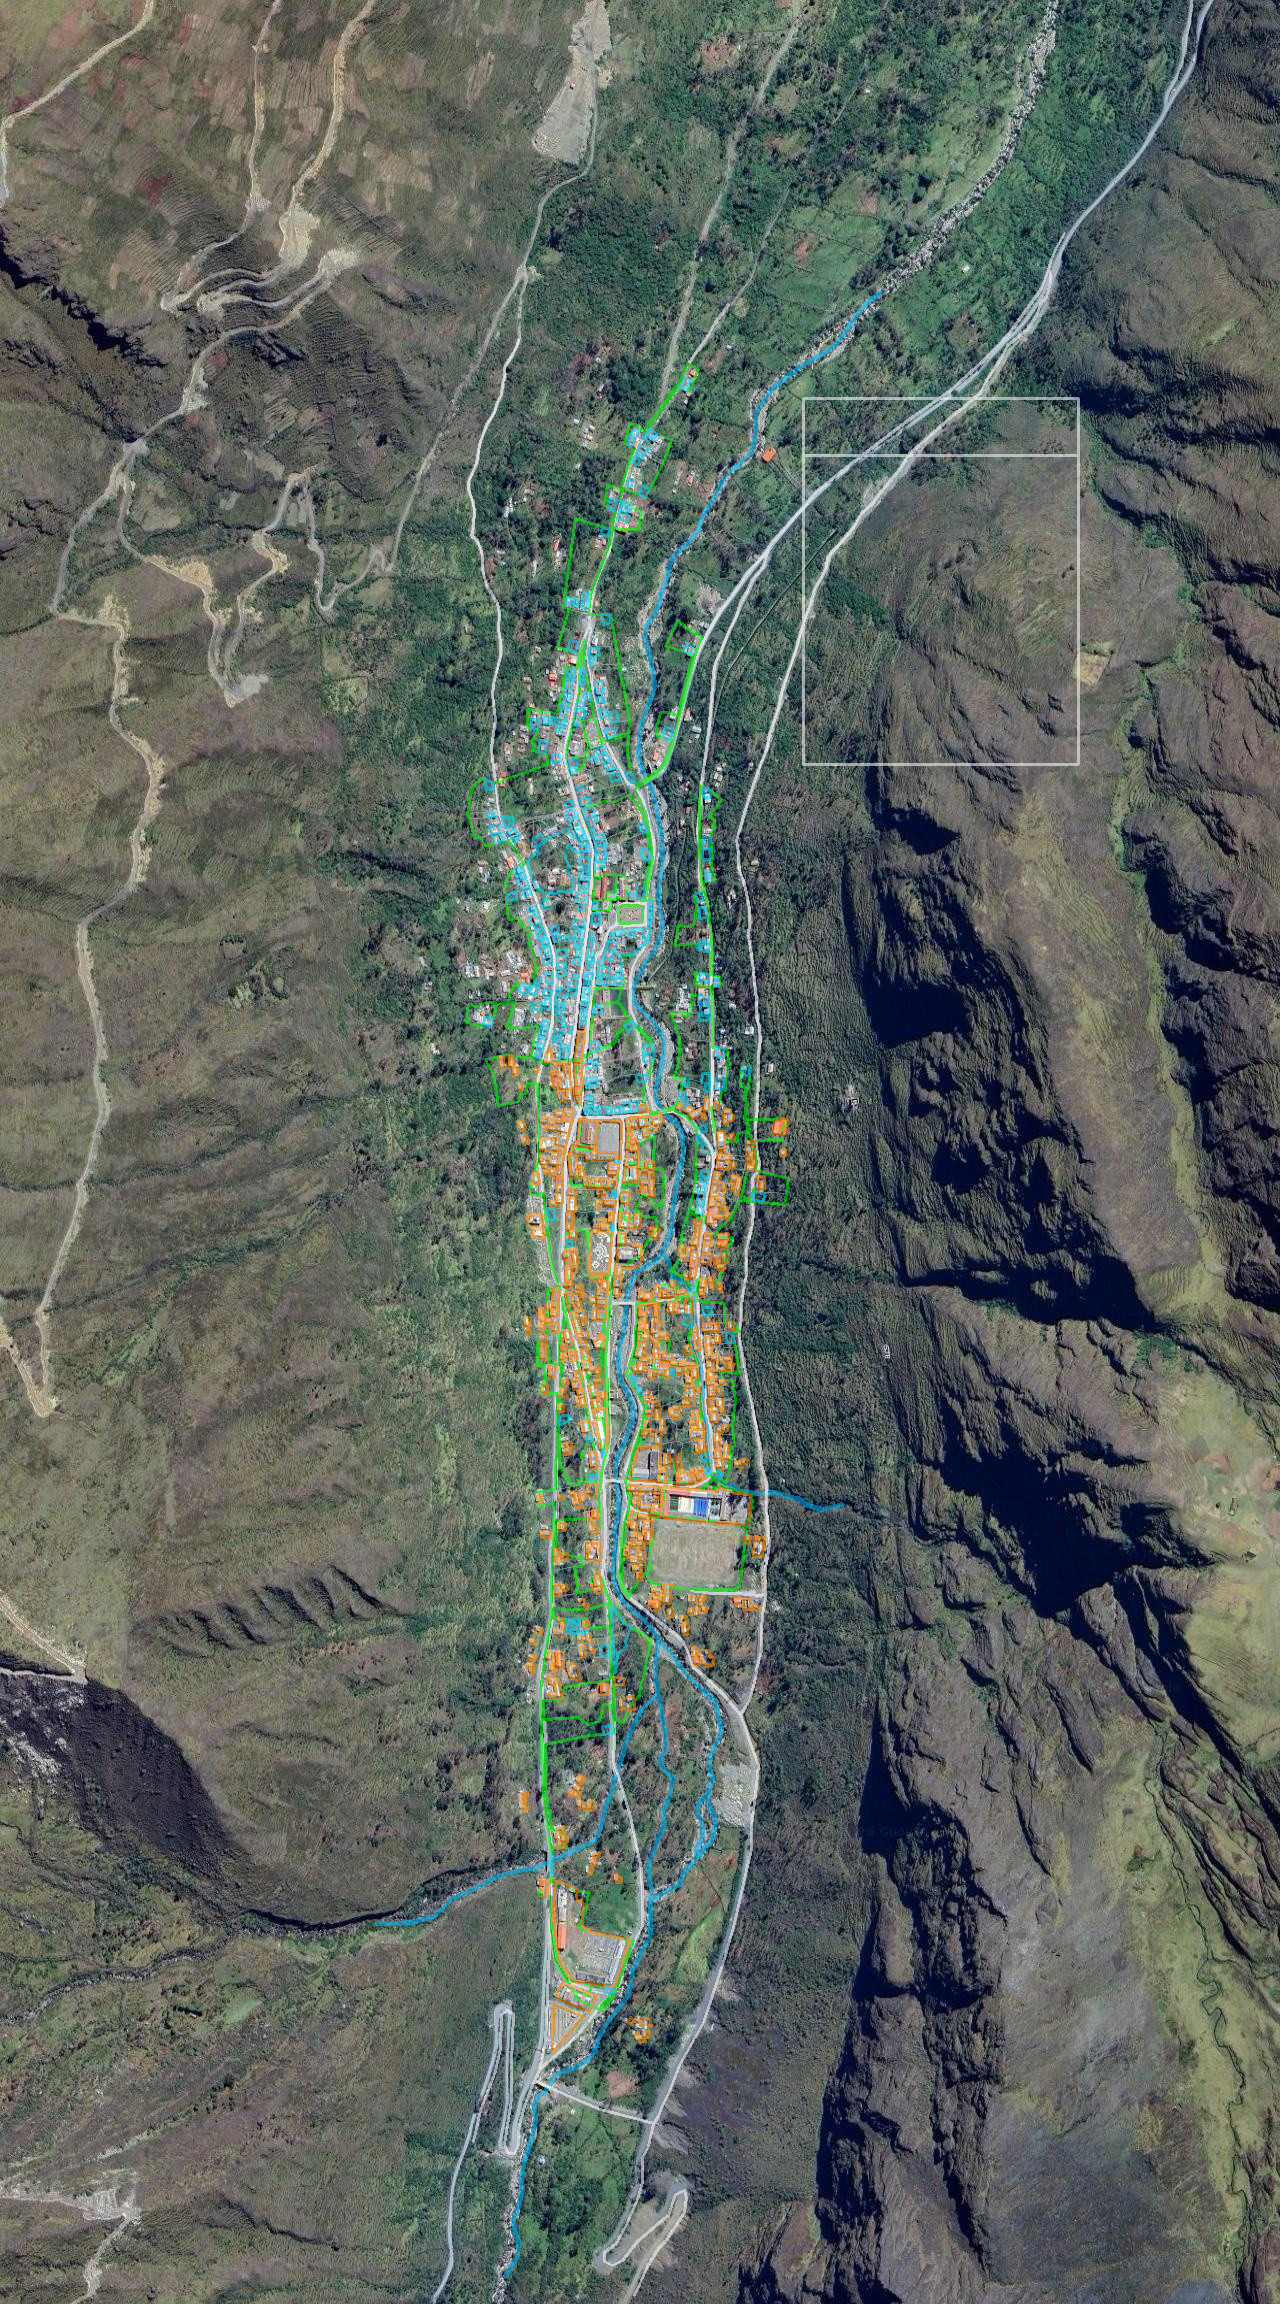
\includegraphics[width=0.85\textwidth,height=0.36\textheight,keepaspectratio]{figuras/01_superposicion_ortofoto_completa.png}
\caption{Superposición ortofotogramétrica y delimitación de manzanas catastrales en Limbani.}
\label{fig:ortofoto}
\end{figure}

\subsection{Modelo Digital Vectorial CAD del Sistema Urbano}
En la Figura~\ref{fig:cad_modelo} se observa la estructura de redes vectoriales que integra las cotas altimétricas, paramentos de predios, alineamientos de vías y cauces fluviales:

\begin{figure}[H]
\centering
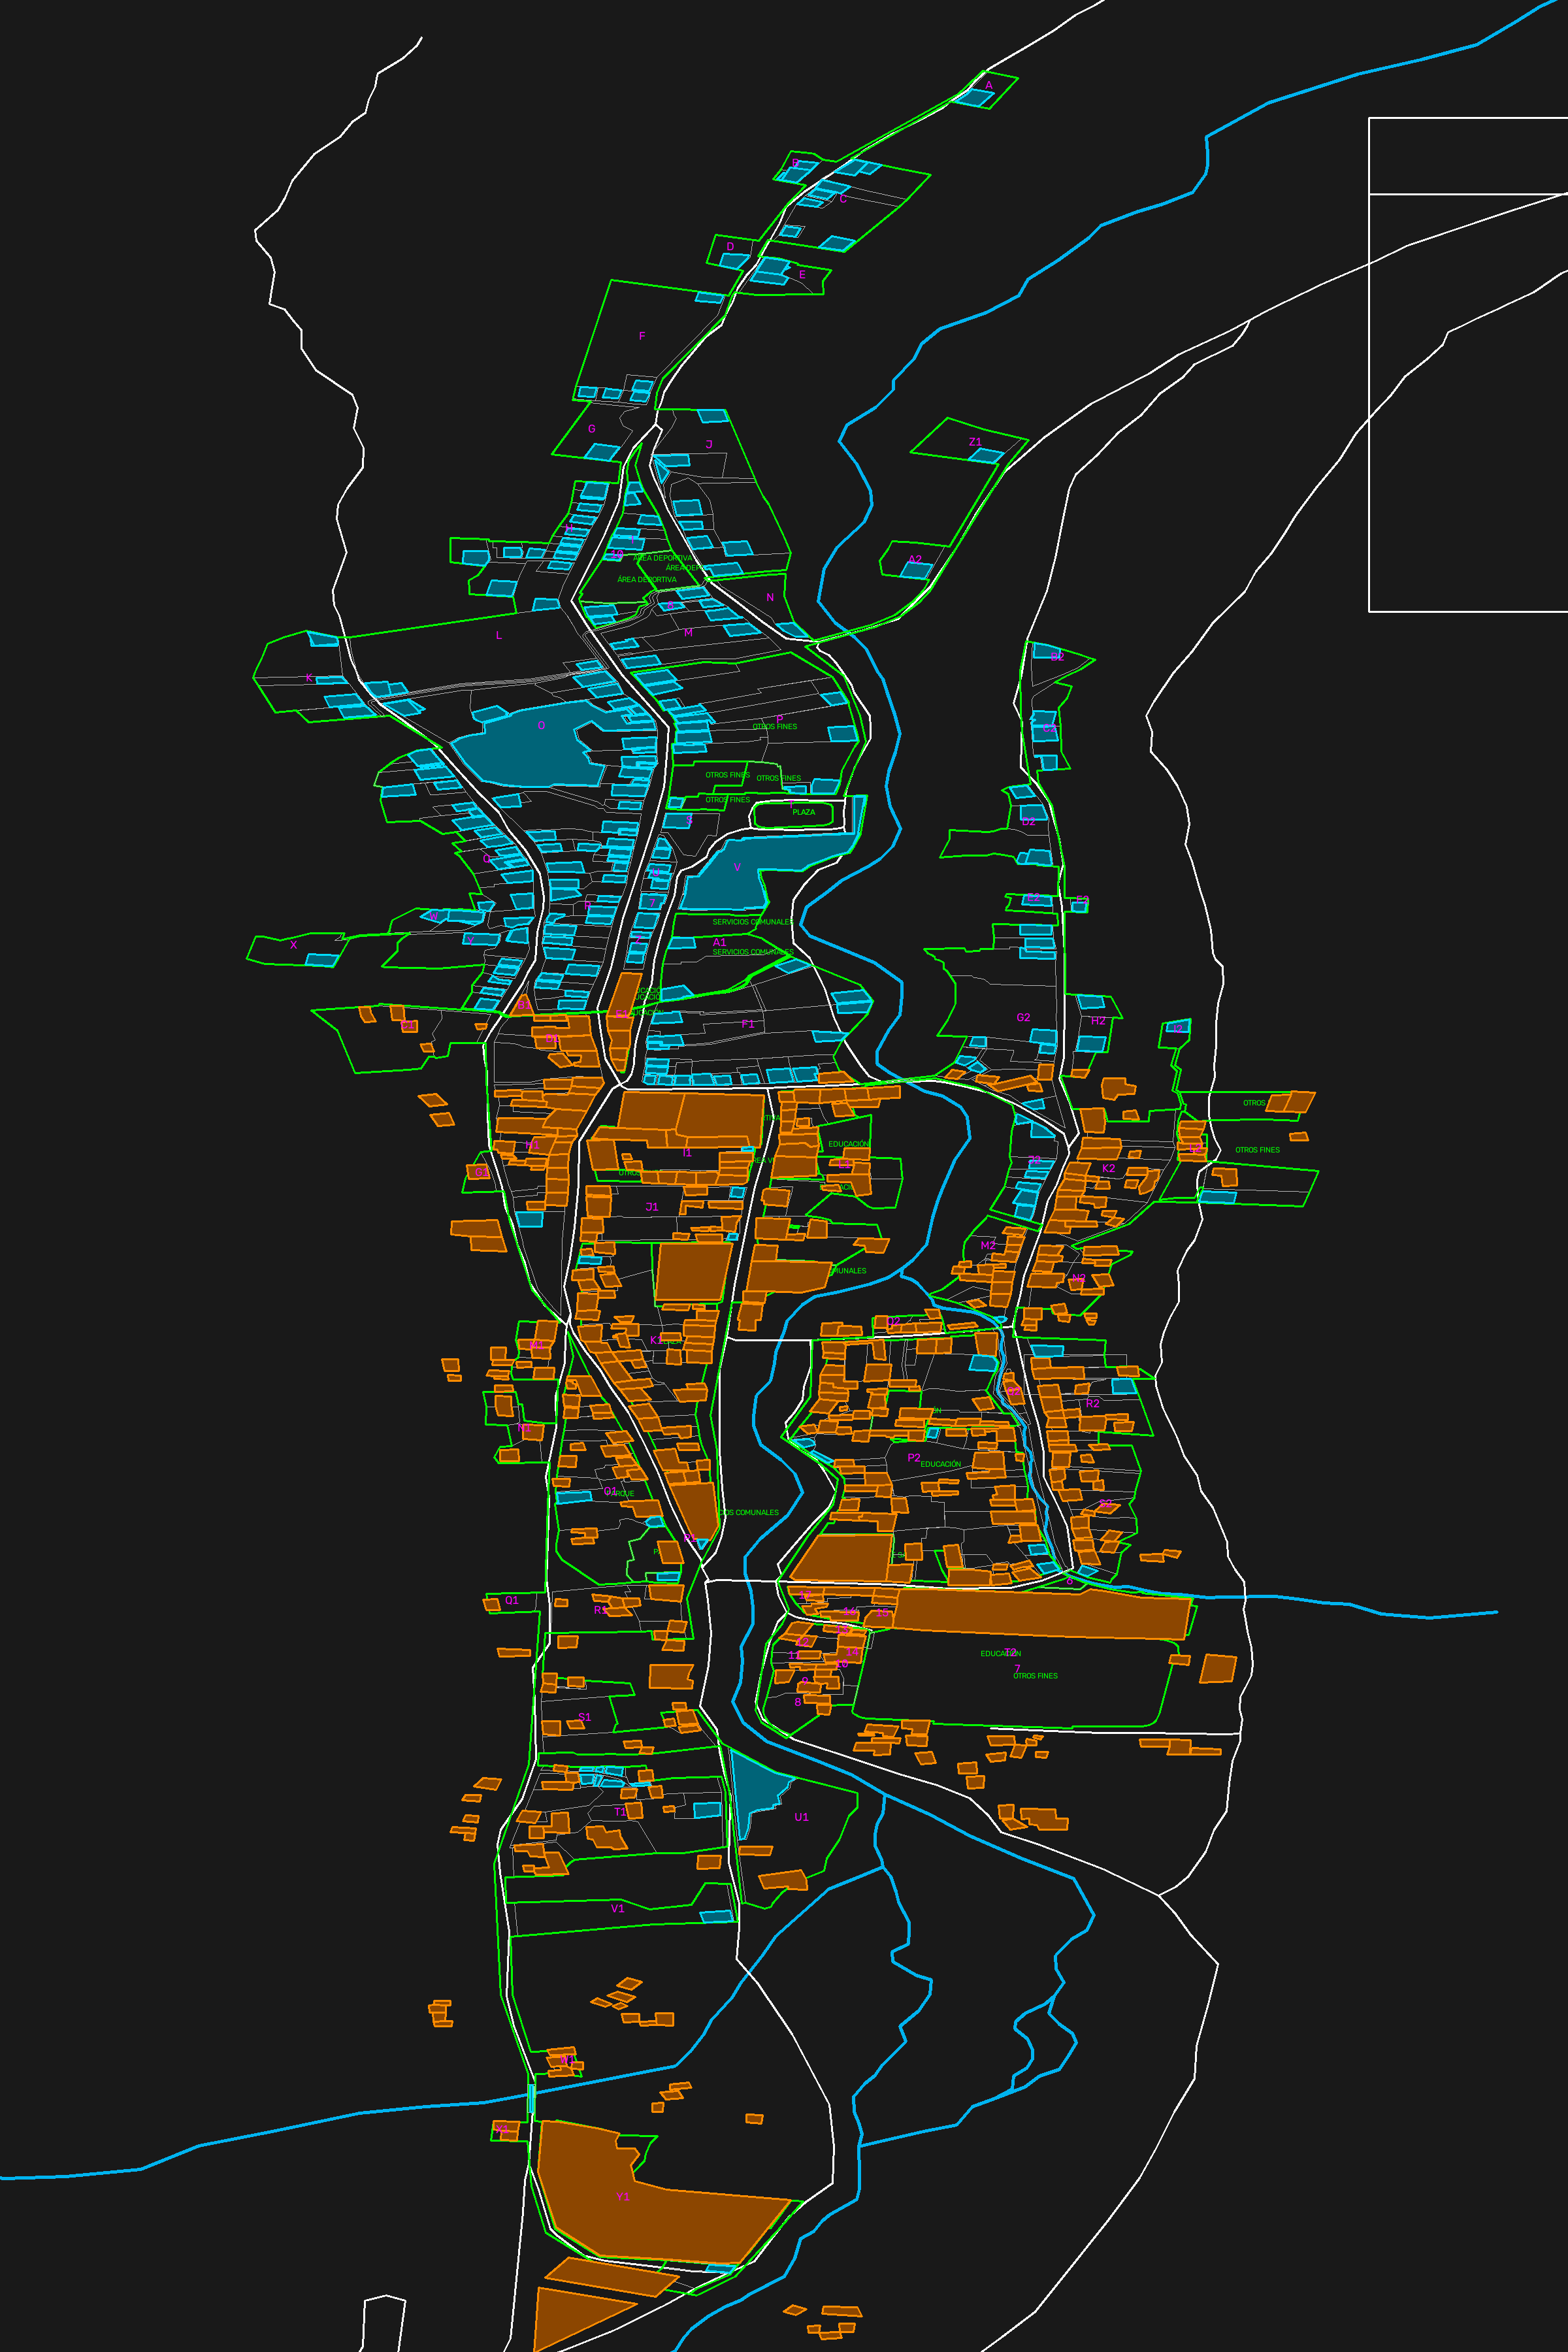
\includegraphics[width=0.85\textwidth,height=0.36\textheight,keepaspectratio]{figuras/02_modelo_autocad_completo.png}
\caption{Modelo geométrico y base catastral vectorial en formato CAD/DXF.}
\label{fig:cad_modelo}
\end{figure}

\newpage
\subsection{Plano General de Redes Eléctricas, Postería y Subestaciones}
La Figura~\ref{fig:redes_detalladas} presenta el diseño electromecánico integrado sobre el catastro oficial de Limbani, mostrando la traza de la línea de 10 kV (rojo), los 24 apoyos de media tensión, las 3 Subestaciones Biposte SED-01, SED-02 y SED-03 (bloques dorados), las retenidas de anclaje (magenta) y los 360 postes de baja tensión (azul) con las 165 luminarias de alumbrado público LED (amarillo):

\begin{figure}[H]
\centering
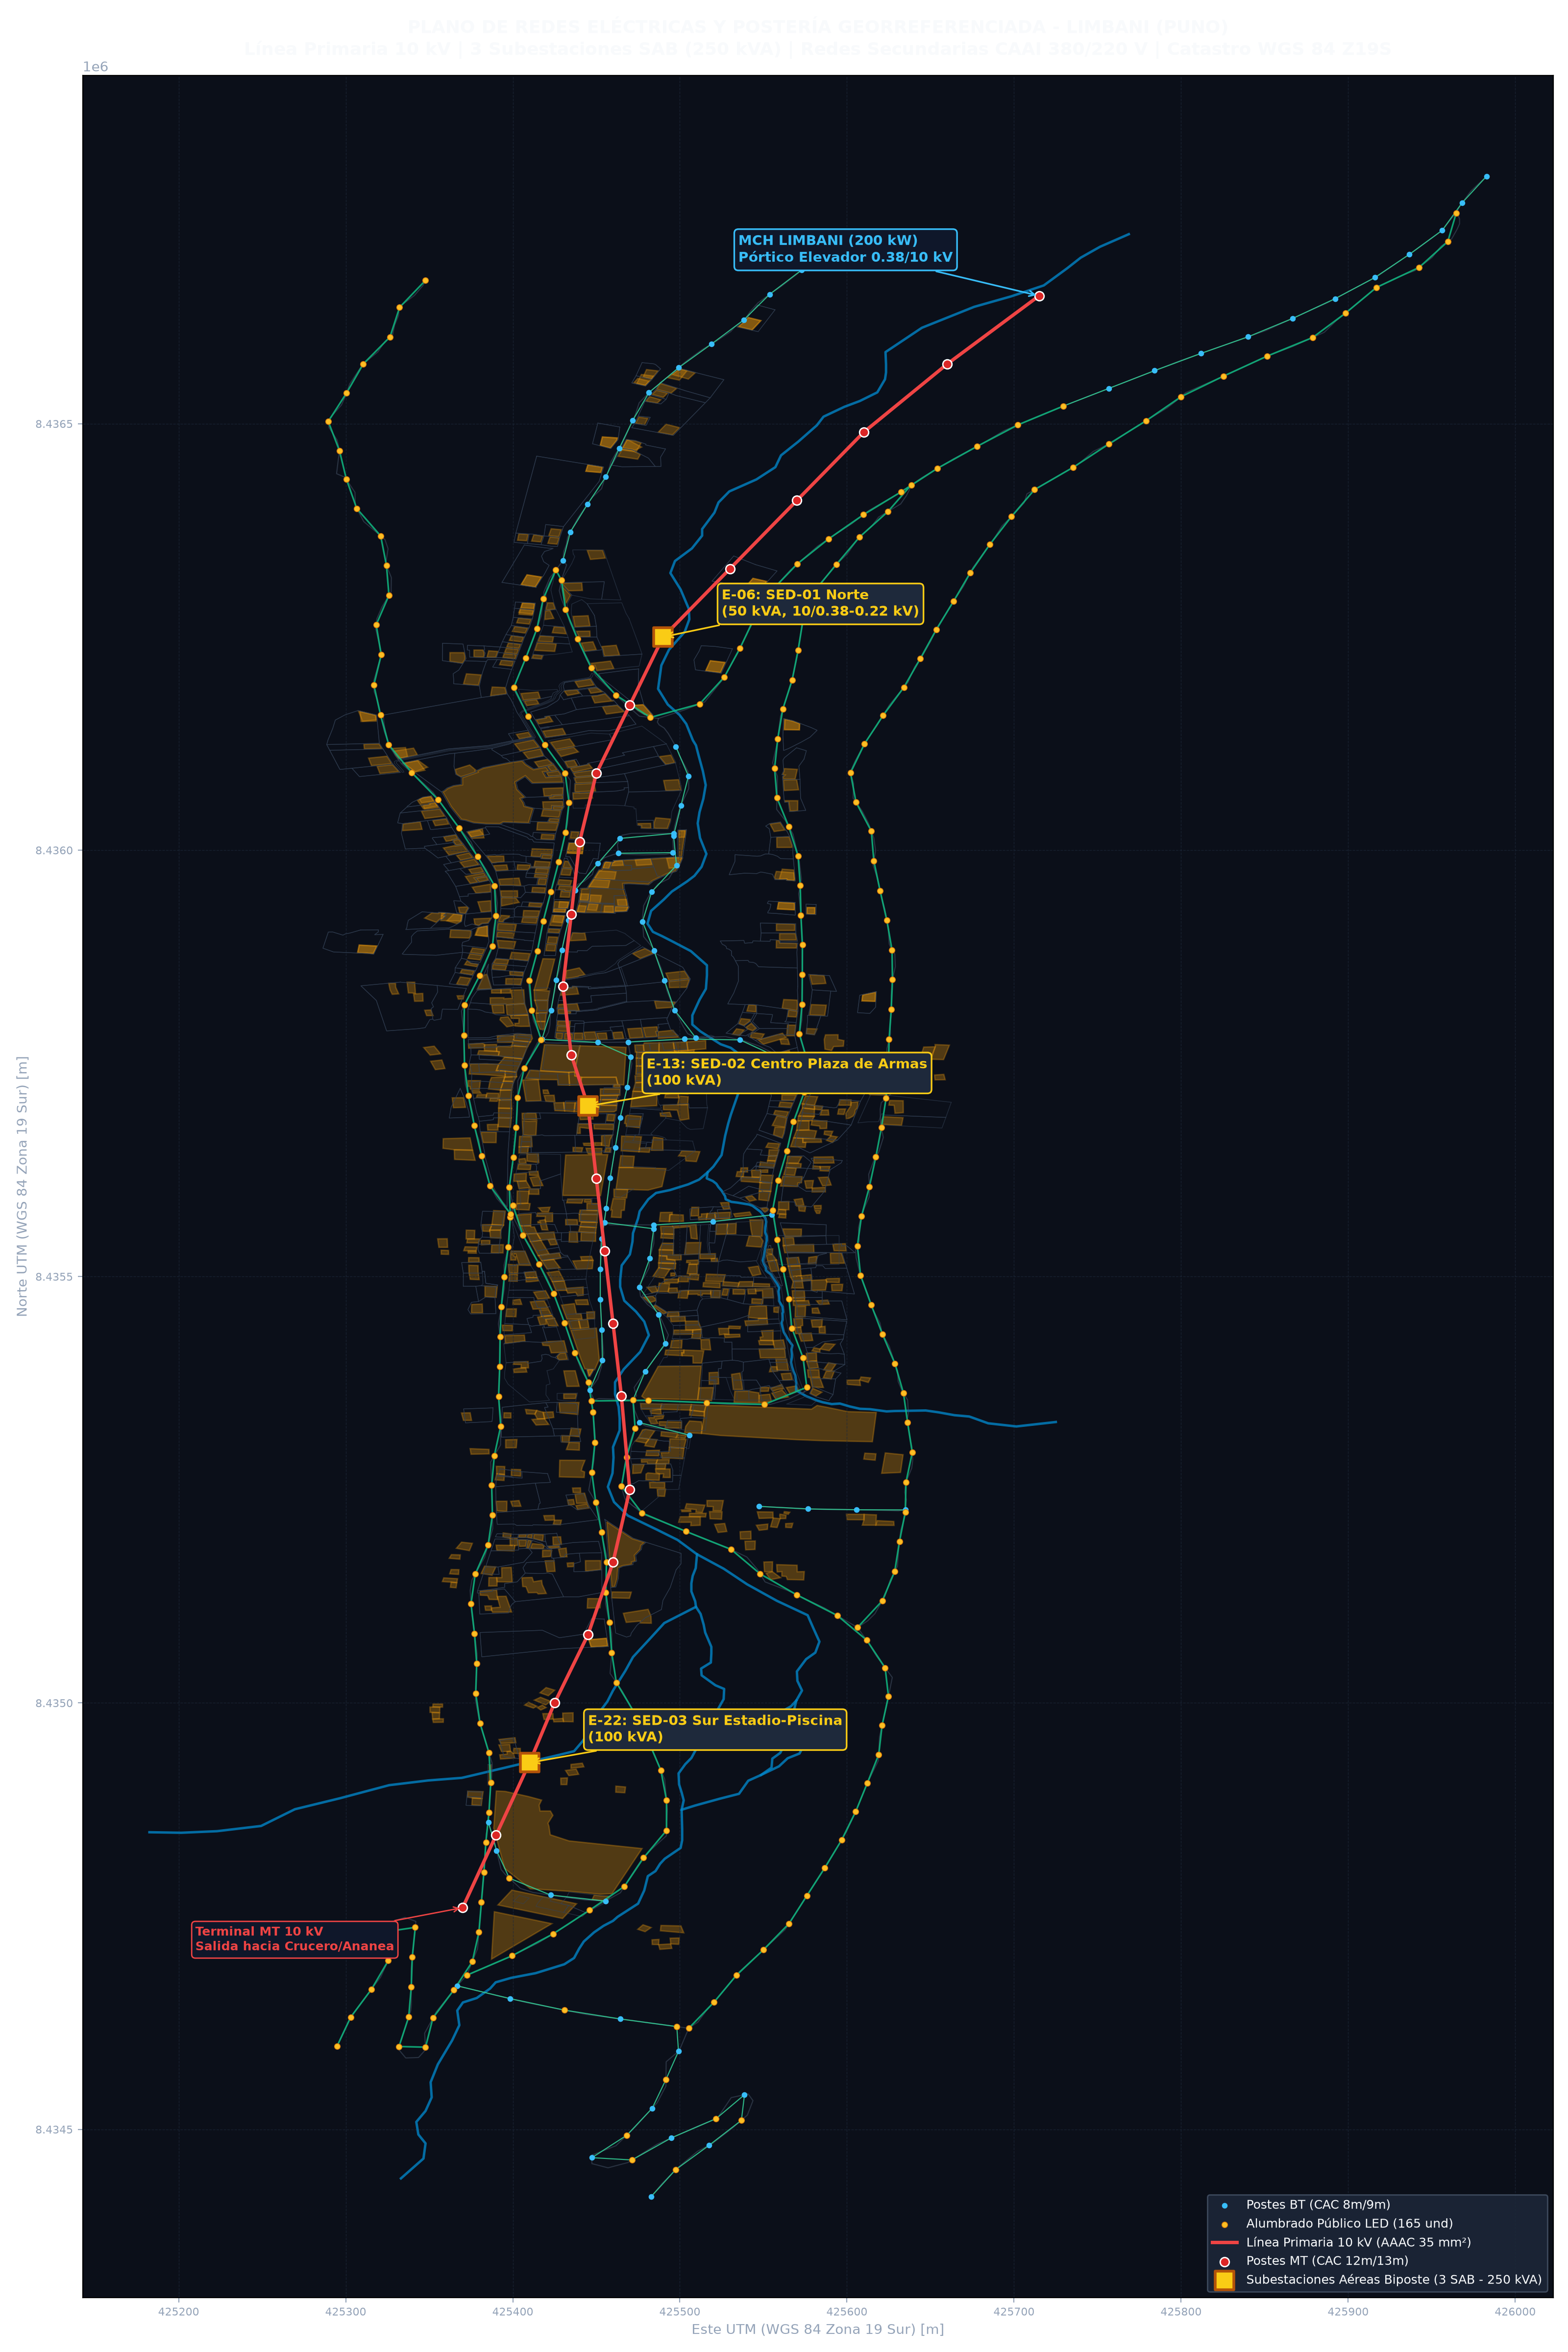
\includegraphics[width=0.85\textwidth,height=0.60\textheight,keepaspectratio]{figuras/07_redes_electricas_detalladas_catastro.png}
\caption{Plano General de Redes Eléctricas, Postería CAC y Subestaciones Aéreas Biposte georreferenciadas en Limbani (WGS 84 Z19S).}
\label{fig:redes_detalladas}
\end{figure}

\newpage
\subsection{Detalle Sector Norte: Casa de Máquinas MCH Limbani y SED-01}
La Figura~\ref{fig:sector_norte} muestra la zona de captación y casa de máquinas de la Minicentral Hidroeléctrica (200 kW con turbina Michell-Banki), el pórtico de salida en 10 kV y la alimentación a la Subestación SED-01 (Norte, 50 kVA) que abastece a 142 lotes:

\begin{figure}[H]
\centering
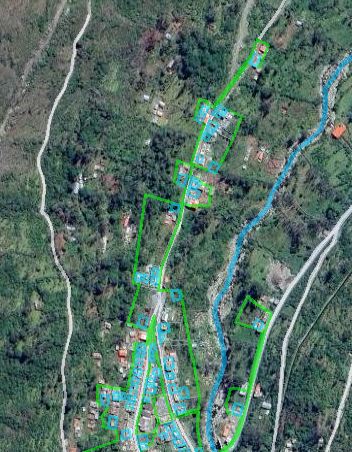
\includegraphics[width=0.85\textwidth,height=0.36\textheight,keepaspectratio]{figuras/03_zoom_sector_norte_hidroelectrica.png}
\caption{Sector Norte: Casa de máquinas MCH Limbani y cobertura de SED-01.}
\label{fig:sector_norte}
\end{figure}

\subsection{Detalle Sector Centro: Plaza de Armas y SED-02}
La Figura~\ref{fig:sector_centro} exhibe el núcleo cívico y comercial de Limbani, donde se emplaza la SED-02 (Centro, 100 kVA) que energiza la Plaza de Armas, Municipalidad, Centro de Salud y 348 lotes de alta densidad:

\begin{figure}[H]
\centering
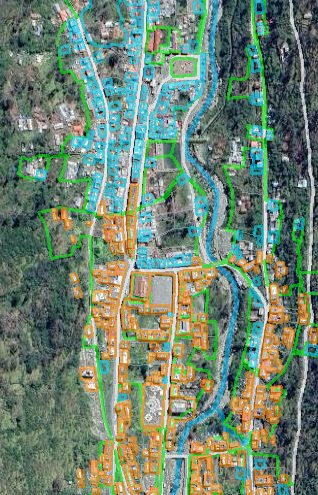
\includegraphics[width=0.85\textwidth,height=0.36\textheight,keepaspectratio]{figuras/04_zoom_sector_centro_plaza_puno.png}
\caption{Sector Centro: Plaza de Armas de Limbani y cobertura de SED-02.}
\label{fig:sector_centro}
\end{figure}

\newpage
\subsection{Detalle Sector Confluencia Fluvial y Estadio Municipal}
La Figura~\ref{fig:sector_confluencia} ilustra la confluencia entre el Río Limbani y la Quebrada Chinchalamani, identificando el cruce aéreo reforzado de media tensión y la derivación hacia el Estadio Municipal:

\begin{figure}[H]
\centering
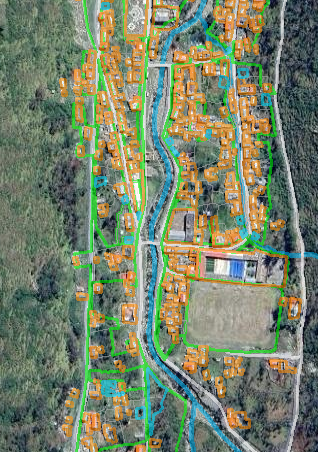
\includegraphics[width=0.85\textwidth,height=0.36\textheight,keepaspectratio]{figuras/05_zoom_sector_confluencia_estadio.png}
\caption{Sector de confluencia fluvial y área de expansión recreacional/deportiva.}
\label{fig:sector_confluencia}
\end{figure}

\subsection{Detalle Sector Sur: Complejo Recreacional, Piscina y SED-03}
La Figura~\ref{fig:sector_sur} presenta la zona sur del casco urbano, correspondiente al sector de la Piscina Municipal y salida hacia Crucero, servido por la Subestación SED-03 (Sur, 100 kVA) para 274 lotes:

\begin{figure}[H]
\centering
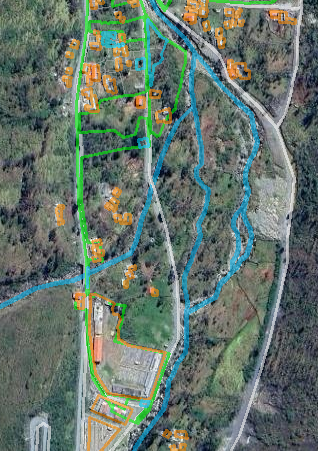
\includegraphics[width=0.85\textwidth,height=0.36\textheight,keepaspectratio]{figuras/06_zoom_sector_sur_piscina_salida.png}
\caption{Sector Sur: Complejo recreacional, piscina y cobertura de SED-03.}
\label{fig:sector_sur}
\end{figure}

\clearpage

\renewcommand{\documentfootertext}{CAPÍTULO VIII: CONCLUSIONES Y BIBLIOGRAFÍA -- LIMBANI}
\chapter*{CAPÍTULO VIII: CONCLUSIONES, RECOMENDACIONES Y BIBLIOGRAFÍA}
\addcontentsline{toc}{chapter}{CAPÍTULO VIII: CONCLUSIONES, RECOMENDACIONES Y BIBLIOGRAFÍA}

\section{CONCLUSIONES TÉCNICAS}

\begin{enumerate}
  \item \textbf{Suficiencia y Viabilidad Energética:} La Minicentral Hidroeléctrica Limbani (MCH Limbani), equipada con una turbina tipo Michell-Banki de flujo transversal y generador síncrono de $200.0\text{ kW}$ ($250.0\text{ kVA}$) a $380\text{ V}$, es plenamente capaz de abastecer la totalidad de la demanda eléctrica del casco urbano consolidado de Limbani. La máxima demanda coincidente calculada para el horizonte de diseño es de $\mathbf{181.80\text{ kW}}$ ($\mathbf{202.00\text{ kVA}}$ a $\cos\phi = 0.90$), lo cual representa un factor de utilización del $\mathbf{90.9\%}$ y deja un margen de reserva operativa del $\mathbf{9.1\%}$ ($18.2\text{ kW}$) para contingencias y pequeños talleres locales.
  \item \textbf{Calidad de Suministro y Perfiles de Tensión:} El diseño electromecánico adoptado garantiza una excelente calidad de tensión en todos los nodos de consumo, superando con holgura los estándares de la Norma Técnica de Calidad de los Servicios Eléctricos (NTCSE):
    \begin{itemize}
      \item En la línea primaria de 10.0 kV ($2.15\text{ km}$, conductor AAAC $35\text{ mm}^2$), la caída de tensión en hora de punta es de apenas $\mathbf{0.504\%}$ ($\Delta V = 50.41\text{ V}$), muy por debajo del límite regulatorio del $5.0\%$.
      \item En la red de baja tensión (380/220 V con cables autoportantes CAAI), la caída de tensión acumulada máxima en el punto más alejado de la SED-02 es de $\mathbf{3.82\%}$, cumpliendo con el valor admisible de $\le 5.0\%$.
    \end{itemize}
  \item \textbf{Alta Eficiencia y Bajas Pérdidas Técnicas:} Las pérdidas por efecto Joule en los $2.15\text{ km}$ de línea primaria en 10 kV ascienden a únicamente $\mathbf{1.05\text{ kW}}$, lo cual representa un insignificante $\mathbf{0.52\%}$ de la energía generada. Esto demuestra la conveniencia técnica de elevar la tensión a 10 kV mediante el transformador elevador de $250\text{ kVA}$ ($0.38/10\text{ kV}$) ubicado en la casa de máquinas, en lugar de realizar una distribución directa en baja tensión que habría resultado inviable por caída de tensión y costo de conductores.
  \item \textbf{Adaptación Climática y Rigor Normativo:} Todo el dimensionamiento de aislamiento, distancias mínimas de seguridad (DMS) y esfuerzos mecánicos en estructuras de concreto armado centrifugado (CAC) ha sido corregido aplicando el factor de derrateo por altitud $k_a = 1.28$ (correspondiente a $3,050\text{ m.s.n.m.}$) y las hipótesis de viento máximo de $90\text{ km/h}$ y temperatura extrema de $-5^\circ\text{C}$ de la Zona 2 (Sierra y Altiplano) del Código Nacional de Electricidad - Suministro 2011.
  \item \textbf{Seguridad de las Personas e Instalaciones:} El sistema de puesta a tierra calculado mediante el modelo de Dwight con dos jabalinas de cobre y tratamiento de bentonita sódica garantiza una resistencia de difusión de $\mathbf{8.14\ \Omega}$ en las tres subestaciones biposte, cumpliendo holgadamente el valor exigido por norma ($\le 10.0\ \Omega$).
  \item \textbf{Presupuesto y Plazo de Ejecución:} El presupuesto estimado referencial de obra asciende a $\mathbf{S/.\ 1,305,876.26}$ (incluyendo gastos generales, utilidad e IGV), con un plazo de ejecución física de $\mathbf{120\text{ días calendario}}$ (4 meses).
\end{enumerate}

\section{RECOMENDACIONES DE OPERACIÓN Y MANTENIMIENTO}

\begin{enumerate}
  \item \textbf{Mantenimiento Preventivo de la Turbina Michell-Banki:} Se recomienda establecer un programa riguroso de inspección trimestral del rodete y los álabes directrices de la turbina cross-flow, especialmente después de las temporadas de lluvias intensas (enero a marzo), a fin de evaluar y corregir el desgaste erosivo producido por sedimentos silíceos arrastrados por las aguas del Río Limbani.
  \item \textbf{Monitoreo Hidrológico en Época de Estiaje:} Durante los meses de mínimo estiaje (julio y agosto), se debe monitorear el caudal entrante al desarenador y cámara de carga de la MCH. En caso de que el caudal baje por debajo de los requerimientos de los 200 kW, se recomienda implementar un plan de gestión de demanda diurna y nocturna, priorizando los servicios esenciales (salud, alumbrado y bombeo de agua).
  \item \textbf{Inspección y Medición de Puestas a Tierra:} Semestralmente y antes del inicio de la temporada de tormentas eléctricas (octubre), se deberán medir las resistencias de los pozos a tierra de las tres subestaciones biposte y de los terminales de baja tensión con telurómetro digital, aplicando reactivación química con bentonita y sales electrolíticas si la resistencia superase los $10\ \Omega$.
  \item \textbf{Desbroce de Servidumbres de Línea en MT:} Mantener despejada la faja de servidumbre de $6.0\text{ m}$ (3.0 m a cada lado del eje de la línea de 10 kV), realizando podas de árboles de eucalipto y arbustos que puedan aproximarse a menos de $2.5\text{ m}$ de los conductores bajo ráfagas de viento.
  \item \textbf{Termografía en Transformadores y Tableros:} Realizar inspecciones termográficas anuales en los bornes de media tensión, bornes secundarios y barras de distribución de los tableros de las subestaciones SED-01, SED-02 y SED-03 para detectar a tiempo falsos contactos o desbalances térmicos.
\end{enumerate}

\section{REFERENCIAS BIBLIOGRÁFICAS Y BASE NORMATIVA}

\begin{enumerate}[label={[\arabic*]}]
  \item \textbf{Ministerio de Energía y Minas del Perú (MEM):} \textit{Código Nacional de Electricidad - Suministro 2011}, aprobado mediante Resolución Ministerial N.° 366-2011-MEM/DM.
  \item \textbf{Dirección General de Electricidad (DGE/MEM):} \textit{Bases para el Diseño de Líneas Primarias en Redes de Distribución}, aprobada por Resolución Directoral N.° 018-2003-EM/DGE.
  \item \textbf{Dirección General de Electricidad (DGE/MEM):} \textit{Bases para el Diseño de Redes Secundarias con Conductores Autoportantes}, aprobada por Resolución Directoral N.° 016-2003-EM/DGE.
  \item \textbf{Dirección General de Electricidad (DGE/MEM):} \textit{Especificaciones Técnicas para el Montaje de Líneas Aéreas y Redes de Distribución}, aprobada por Resolución Directoral N.° 026-2003-EM/DGE.
  \item \textbf{Ministerio de Energía y Minas del Perú:} \textit{Norma Técnica de Calidad de los Servicios Eléctricos (NTCSE)}, aprobada por Decreto Supremo N.° 020-97-EM y sus modificatorias.
  \item \textbf{Ministerio de Energía y Minas del Perú:} \textit{Reglamento de Seguridad y Salud en el Trabajo con Electricidad (RESESATE)}, aprobado por Resolución Ministerial N.° 111-2013-MEM/DM.
  \item \textbf{Instituto Nacional de Calidad (INACAL):} \textit{NTP 370.258: Conductores de aleación de aluminio para líneas aéreas (AAAC)}.
  \item \textbf{Instituto Nacional de Calidad (INACAL):} \textit{NTP 370.254: Cables concéntricos trenzados para distribución aérea (CAAI)}.
  \item \textbf{Instituto Nacional de Calidad (INACAL):} \textit{NTP 339.027: Postes de hormigón (concreto) armado para líneas aéreas}.
  \item \textbf{Instituto Nacional de Calidad (INACAL):} \textit{NTP 370.002: Transformadores de potencia. Especificaciones y pruebas}.
  \item \textbf{International Electrotechnical Commission (IEC):} \textit{IEC 60076: Power Transformers}; \textit{IEC 60502: Power cables with extruded insulation}; \textit{IEC 61089: Round wire concentric lay overhead electrical stranded conductors}.
  \item \textbf{Municipalidad Distrital de Limbani:} \textit{Catastro Urbano Oficial y Base Georreferenciada WGS 84 Zona 19 Sur}, 2026.
\end{enumerate}


\end{document}
